%*****************************************
\chapter{Presenting Data With Charts}\label{ch04:charts}
%*****************************************

One of the most important things to consider when using charts in Excel is that they are intended to be used for communicating an idea to an audience, whether that audience is reading a written report or listening to a presentation. In fact, Excel charts are often imported or pasted into Word documents or PowerPoint slides, which serve the purpose of communicating ideas to an audience. Although there are no rules set in stone for using specific charts for certain data types, some chart types are designed to communicate certain messages better than others. This chapter explores numerous charts that can be used for a variety of purposes. In addition, the chapter examines formatting charts and using those charts in Word and PowerPoint documents.

\section{Choosing a Chart Type}

\begin{center}
	\begin{objbox}{Learning Objectives}
		\begin{itemize}
			\setlength{\itemsep}{0pt}
			\setlength{\parskip}{0pt}
			\setlength{\parsep}{0pt}

			\item Construct a line chart to show a time series trend.
			\item Learn how to adjust the Y axis scale.
			\item Construct a line chart to present a comparison of two trends.
			\item Learn how to use a column chart to show a frequency distribution.
			\item Create a separate chart sheet for a chart embedded in a worksheet.
			\item Construct a column chart that compares two frequency distributions.
			\item Learn how to use a pie chart to show the percent of total for a data set.
			\item Construct a stacked column chart to show how a percent of total changes over time.
			
		\end{itemize}
	\end{objbox}
\end{center}

This section reviews the most commonly used Excel chart types. To demonstrate the variety of chart types available in Excel, it is necessary to use a variety of data sets. This is necessary not only to demonstrate the construction of charts but also to explain how to choose the right type of chart given the data and idea being communicated.

Here are a few key points to consider before creating any chart in Excel.

\begin{enumerate}
	\item The first is identifying the idea or message. It is important to keep in mind that the primary purpose of a chart is to present quantitative information to an audience. Therefore, first decide what message or idea is being presented. This is critical in selecting specific data from a worksheet that will be used in a chart. This chapter continually reinforces the idea of determining the intended message before creating each chart.
	\item The second key point is selecting the right chart type. The chart type selected will depend on the data and the message to communicate.
	\item The third key point is identifying the values that should appear on the X and Y axes. One of the ways to identify which values belong on the X and Y axes is to sketch the chart on paper first. Visualizing the chart first makes easier to select the information and then use Excel to construct an effective chart that accurately communicates the message. 
\end{enumerate}

Table \ref{04:tab01}, \textit{Key Steps Before Constructing an Excel Chart}, provides a brief summary of the preceding points.

\begin{table}[H]
	\rowcolors{1}{}{tablerow} % zebra striping background
	{\small
		%\fontsize{8}{10} \selectfont %Replace small for special font size
		\begin{longtable}{L{0.75in}L{3.50in}} %Left-aligned, Max width: 4.25in
			\textbf{Step} & \textbf{Description} \endhead
			\hline
			Define the message & Identify the main idea being communicated. If there is no main point or important message that can be revealed by a chart then do not create a chart.\\
			Identify the data needed & Once there is a clear message, identify the data on a worksheet that is needed to construct a chart. In some cases, formulas may be needed to better define the data or some data items may need to be consolidated into broader categories.\\
			Select a chart type & The type of chart selected will depend on the message being communicated and the data being presented.\\
			Identify the values for the X and Y axes & After selecting a chart type, drawing a sketch is often helpful in identifying which values should be on the X and Y axes. In Excel, the axes are: the ``category'' axis, which is usually the horizontal axis, where the labels are found, and the ``value'' axis, which is usually the vertical axis, where the numbers are found.\\
			\rowcolor{captionwhite}
			\caption{Key Steps before Constructing an Excel Chart}
			\label{04:tab01}
		\end{longtable}
	} % End small
\end{table}

\subsection{Time Series Trend: Line Chart 1}

The first chart is a line chart. Figure \ref{04:fig01} shows part of the data that will be used to create two line charts. The first will show the trend of the NASDAQ stock index.

\footnote{The NASDAQ data was found at \url{http://www.investopedia.com/terms/n/nasdaq.asp}}

This chart will be used to communicate a simple message: to show how the index has performed over a two-year period. This chart can be used in a presentation to show whether stock prices have been increasing, decreasing, or remaining constant over the designated period of time.

\begin{center}
	\begin{infobox}{Integrity Check}
		\textbf{Carefully Select Data When Creating a Chart}
		\\
		\\
		Just because a worksheet contains data does not mean it must all be placed onto a chart. When creating a chart, it is common for only specific data points to be used. To determine what data should be used when creating a chart, start by identifying the message or idea that must be communicated to the audience.
	\end{infobox}
\end{center}

\begin{figure}[H]
	\centering
	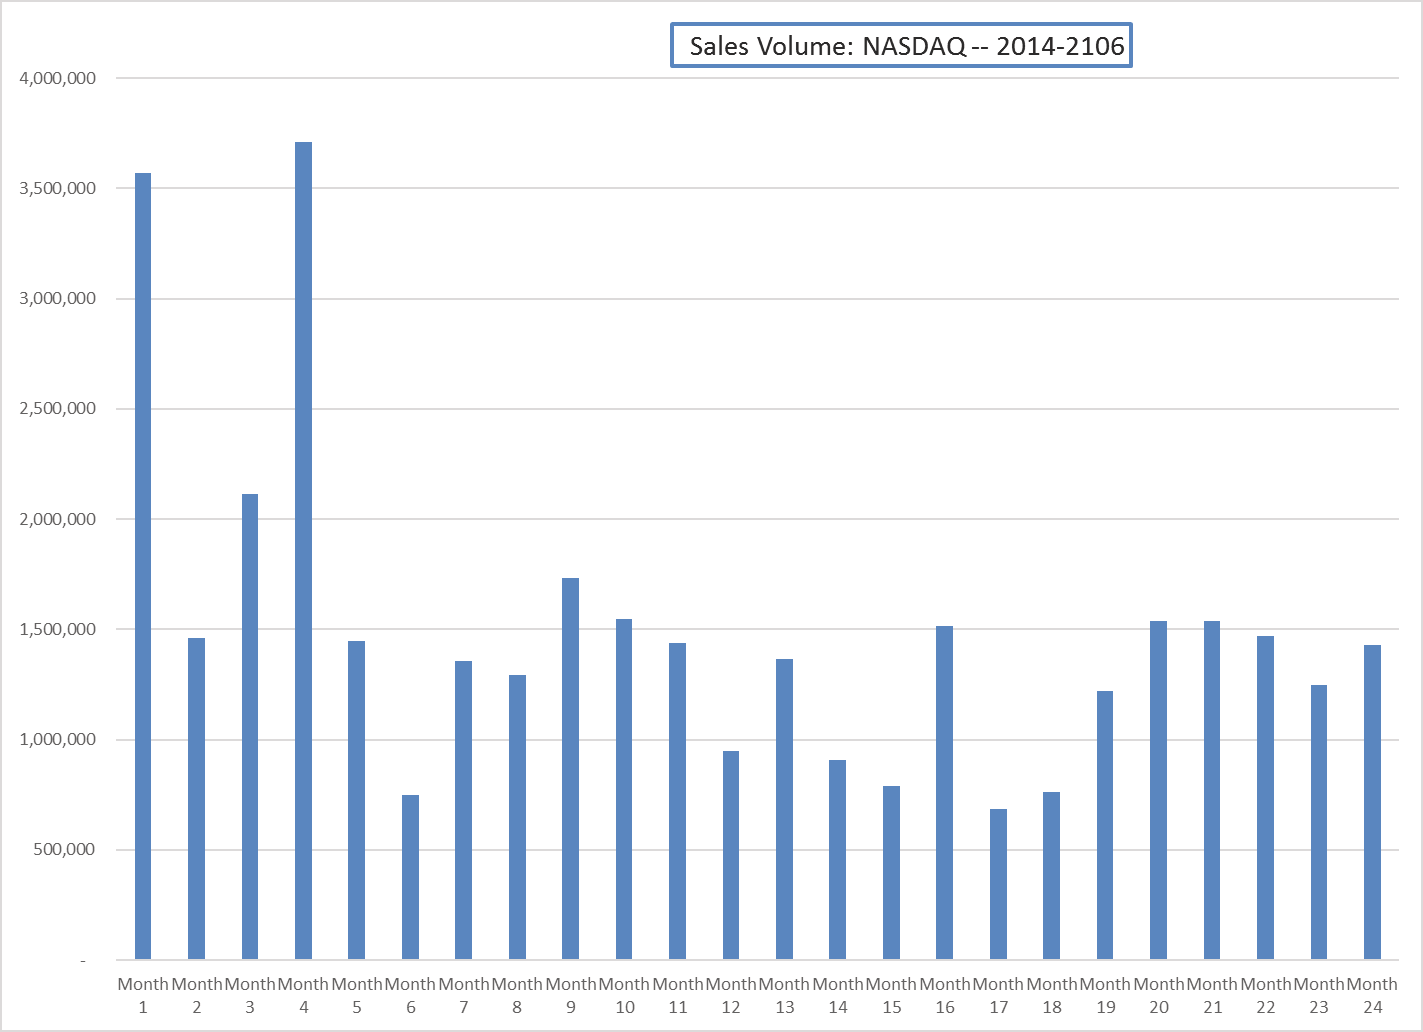
\includegraphics[width=\maxwidth{.95\linewidth}]{gfx/ch04_fig01}
	\caption{Stock Trends}
	\label{04:fig01}
\end{figure}

Before creating the line chart, it is important to identify why it is an appropriate chart type given the message being communicated and the data available. When presenting the trend for any data over a designated period of time, the most commonly used chart types are the line chart and the column chart. A column chart is limited to a certain number of bars or data points. As the number of bars increases it becomes increasingly difficult to read. The worksheet contains $ 24 $ points of data that were used to construct the chart shown in Figure \ref{04:fig01}. This is generally too many data points to put on a column chart, which is why a line chart is a better choice. The line chart will show the volume of sales for the NASDAQ on the Y axis and the Month number on the X axis. The following steps explain how to construct this chart.

\textit{Data file: CH4 Data}

\begin{enumerate}
	\item Open data file \fmtWorkbookName{CH4 Data} and save it as \fmtWorkbookName{CH4 Charting}.
	\item Navigate to the \fmtWorksheetName{Stock Trend} worksheet.
	\item Highlight the range \fmtCellLocation{B4:C28} on the \fmtWorksheetName{Stock Trend} worksheet. (Note that a label in the first row and more labels in column B are selected. Note where they show up in the completed chart.)
	\item Click the \fmtRibbonTab{Insert} tab of the ribbon.
	\item Click the \fmtRibbonButton{Line} button in the \fmtRibbonGroup{Charts} group of commands. Click the first option from the list, which is a basic 2D Line Chart (see Figure \ref{04:fig02}).
\end{enumerate}

\begin{figure}[H]
	\centering
	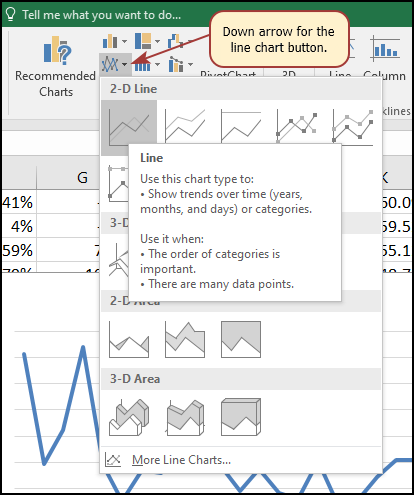
\includegraphics[width=\maxwidth{.95\linewidth}]{gfx/ch04_fig02}
	\caption{Selecting the Basic Line Chart}
	\label{04:fig02}
\end{figure}

This adds, or embeds, the line chart to the worksheet, as shown in Figure \ref{04:fig03}. Notice where the labels showed up on the chart.

\begin{center}
	\begin{infobox}{Why?}
		\textbf{Line Chart vs. Column Chart}
		\\
		\\
		Both a line chart and a column chart can be used to illustrate a trend over time. However, a line chart is far more effective when there are many periods of time being measured. For example, if fifty-two weeks are being reported a column chart would require fifty-two bars. A general rule of thumb is to use a column chart when twenty bars or fewer are required. A column chart becomes difficult to read as the number of bars exceeds twenty.
	\end{infobox}
\end{center}

Notice that additional tabs, called ``contextual'' tabs, are added to the ribbon when a chart is selected and only appear when the chart is active. The commands in these tabs will be demonstrated throughout this chapter.

\begin{figure}[H]
	\centering
	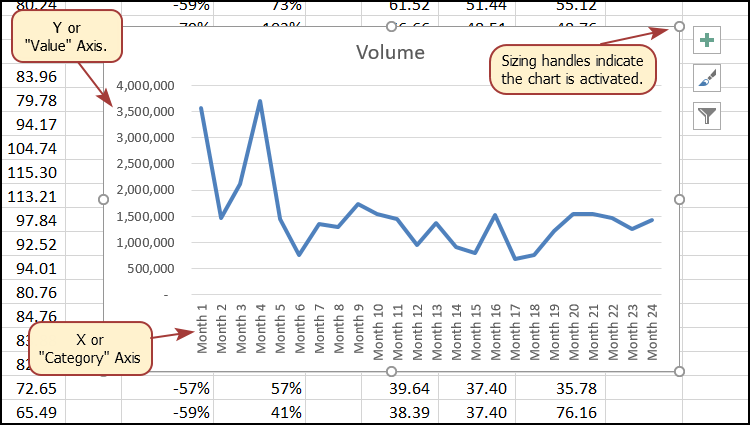
\includegraphics[width=\maxwidth{.95\linewidth}]{gfx/ch04_fig03}
	\caption{Embedded Line Chart in the Stock Trend Worksheet}
	\label{04:fig03}
\end{figure}

As shown in Figure \ref{04:fig03}, the embedded chart is not placed in an ideal location on the worksheet since it is covering several cell locations that contain data. The following steps demonstrate common adjustments that are made when working with embedded charts.

\begin{enumerate}
	\item \textbf{Moving a chart}: Click and drag the upper left corner of the chart to the corner of cell \fmtCellLocation{B30}.
	\item \textbf{Resizing a chart}: Place the mouse pointer over the right upper corner sizing handle, hold down the \fmtKeystroke{Alt} key on the keyboard, and click and drag the chart so it ``snaps'' to the right side of Column I.
	\item Repeat step 2 to resize the chart so the top ``snaps'' to the top of Row $ 30 $, the bottom ``snaps'' to the bottom of Row $ 45 $, and the left side ``snaps'' to the left side of Column B. Make sure the right side of the chart snaps to the line between column I and J.
	\item \textbf{Adjusting the chart title}: Click the chart title once. Then click in front of the first letter. This should place a blinking cursor in front of the letter which allows the title of the chart to be modified. Type the following in front of the first letter in the chart title: \fmtTyping{May 2014-2016 Trend for NASDAQ Sales}.
	\item Click anywhere outside of the chart to deactivate it.
	\item Save the worksheet.
\end{enumerate}

\begin{center}
	\begin{infobox}{Note}
		\textbf{Contextual Tabs}
		\\
		Excel $ 2010 $ uses three contextual tabs for charts. Later versions use only two. Each version has the same tools, they are just organized a little differently.\\
	\end{infobox}
\end{center}

Figure \ref{04:fig04} shows the line chart after it is moved and resized. Notice that the title of the chart has been edited to read \fmtTyping{May 2014-2016 Trend for NASDAQ Sales Volume}. Notice that the sizing handles do not appear around the perimeter of the chart. This is because the chart has been deactivated. To activate the chart, click anywhere inside the chart perimeter.

\begin{tabular}{p{3.25in}p{0.5in}} %Max width: 4.25in
	\hline
	\textit{Note:} The pointer will change into the shape illustrated on the right when it is in the right place to \textbf{move} the chart. & \raisebox{-0.30in}{
\includegraphics[]{gfx/ch04_fig99}} \\
	\hline
	\textit{Note:} The pointer will change into the shape illustrated on the right when it is in the right place to \textbf{resize} the chart. & \raisebox{-0.30in}{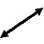
\includegraphics[]{gfx/ch04_fig98}} \\
	\hline
\end{tabular}

\begin{figure}[H]
	\centering
	
\includegraphics[width=\maxwidth{.95\linewidth}]{gfx/ch04_fig04}
	\caption{Line Chart Moved and Resized}
	\label{04:fig04}
\end{figure}

\begin{center}
	\begin{sklbox}{Skill Refresher}
		\textbf{Inserting a Line Chart}
		\\
		\begin{itemize}
			\setlength{\itemsep}{0pt}
			\setlength{\parskip}{0pt}
			\setlength{\parsep}{0pt}

			\item Highlight a range of cells that contain data that will be used to create the chart. Be sure to include labels in the selection.
			\item Click the \fmtRibbonTab{Insert} tab of the ribbon.
			\item Click the \fmtRibbonButton{Line} button in the \fmtRibbonGroup{Charts} group.
			\item Select a format option from the \fmtPopupBox{Line Chart} drop-down menu.
			
		\end{itemize}
	\end{sklbox}
\end{center}

\begin{center}
	\begin{infobox}{Integrity Check}
		\textbf{Category Axis}
		\\
		\\
		When using line charts in Excel, keep in mind that anything placed on the X axis is considered a descriptive label, not a numeric value. This is an example of a category axis. This is important because there will never be a change in the spacing of any items placed on the X axis of a line chart. If numeric data must be placed on the category axis, the chart will need to be modified, which is covered later in the chapter.		
	\end{infobox}
\end{center}

\subsubsection{Adjusting the Y Axis Scale}

After creating an Excel chart, it may be necessary to adjust the scale of the Y axis. Excel automatically sets the maximum value for the Y axis based on the data used to create the chart and the minimum value is usually set to zero. That is usually appropriate. However, depending on the data used to create the chart, setting the minimum value to zero can substantially minimize the graphical presentation of a trend. For example, the trend shown in Figure \ref{04:fig04} appears to be increasing slightly in recent months. The presentation of this trend can be improved if the minimum value started at $ 500,000 $. The following steps explain how to make this adjustment to the Y axis.

\begin{enumerate}
	\item Click anywhere on the Y (value or vertical) axis on the \fmtPopupBox{May 2014-2016 Trend for NASDAQ Sales Volume} line chart in the \fmtWorksheetName{Stock Trend} worksheet.
	\item Right Click and select \fmtPopupButton{Format Axis}. The \fmtPopupBox{Format Axis Pane} should appear, as shown in Figure \ref{04:fig05}. \textit{Note}: If \fmtPopupButton{Format Axis} is not on the menu then the mouse was clicked in the wrong location. Press \fmtKeystroke{Escape} to turn the menu off and try again.
\end{enumerate}

\begin{figure}[H]
	\centering
	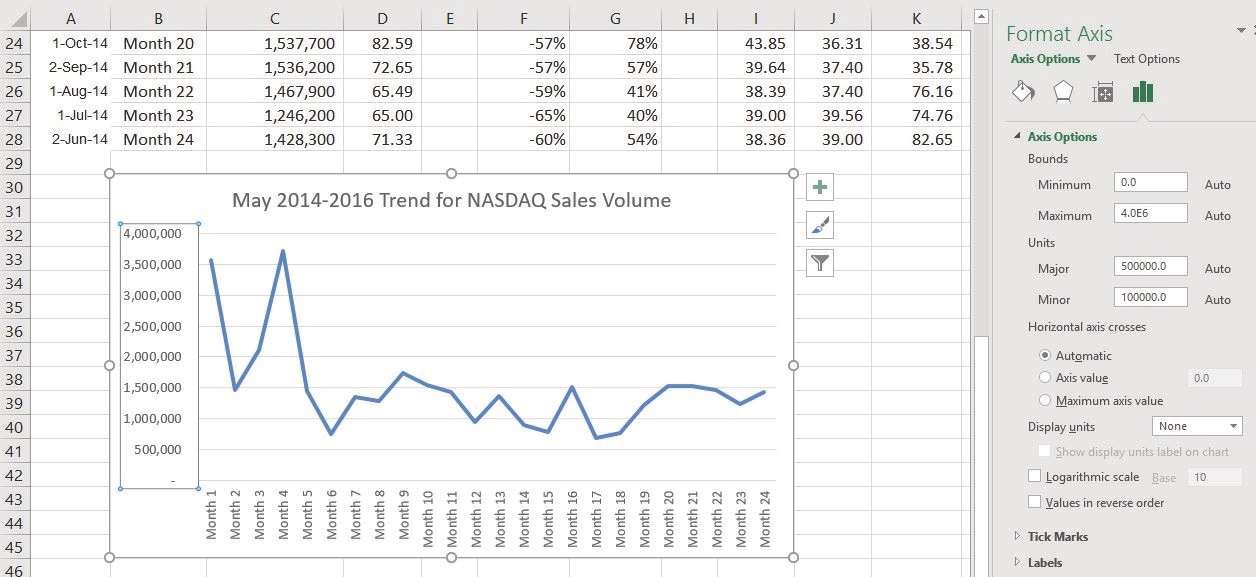
\includegraphics[width=\maxwidth{.95\linewidth}]{gfx/ch04_fig05}
	\caption{Format Axis Pane}
	\label{04:fig05}
\end{figure}

\begin{enumerate}[resume]
	\item In the \fmtPopupBox{Format Axis} pane, click the input box for the \fmtPopupBox{Minimum} axis option and delete the zero. Then type the number $ 500000 $ and press \fmtKeystroke{Enter}. As soon as this change is made the Y axis on the chart adjusts.
	\item Click the \fmtPopupButton{X} in the upper right corner of the \fmtPopupBox{Format Axis} pane to close it.
	\item Save the workbook.
\end{enumerate}

Figure \ref{04:fig06} shows the change in the presentation of the trend line. Notice that with the Y axis starting at $ 500,000 $, the trend for the NASDAQ is more pronounced. This adjustment makes it easier for the audience to see the magnitude of the trend. Do be careful when adjusting the Y axis. It is easy to distort a relatively small trend to make it look bigger than it really is.

\begin{figure}[H]
	\centering
	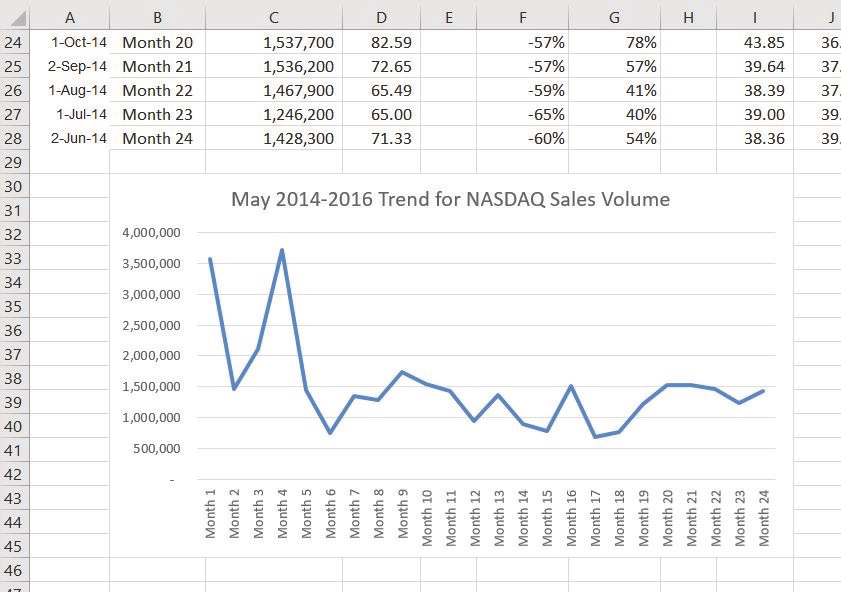
\includegraphics[width=\maxwidth{.95\linewidth}]{gfx/ch04_fig06}
	\caption{Adjusted Y Axis for the S\&P 500 Chart}
	\label{04:fig06}
\end{figure}

\begin{center}
	\begin{sklbox}{Skill Refresher}
		\textbf{Adjusting the Y Axis Scale}
		\\
		\begin{itemize}
			\setlength{\itemsep}{0pt}
			\setlength{\parskip}{0pt}
			\setlength{\parsep}{0pt}

			\item Click anywhere along the Y axis to activate it.
			\item Right Click. (\textit{Note}: the \fmtRibbonTab{Format} tab can also be selected in the \fmtRibbonGroup{Chart Tools} section of the ribbon.)
			\item Select \fmtRibbonButton{Format Axis}
			\item In the \fmtPopupBox{Format Axis} pane, make the changes to the Axis Options.
			\item Click in the input box next to the desired axis option and then type the new scale value.
			\item Click the \fmtPopupButton{Close} button at the top right of the \fmtPopupBox{Format Axis} pane to close it.
			
		\end{itemize}
	\end{sklbox}
\end{center}

\subsection{Trend Comparisons: Line Chart 2}

A second line chart will be created using the data in the \fmtWorksheetName{Stock Trend} worksheet. The purpose of this chart is to compare two trends: the change in volume for the NASDAQ and the change in the Closing price.

Before creating the chart to compare the NASDAQ volume and sales price, it is important to review the data in the range \fmtCellLocation{B4:D28} on the \fmtWorksheetName{Stock Trend} worksheet. The volume of sales and closing price cannot be used because the values are not comparable. That is, the closing price is in a range of $ \$45.00 $ to $ \$115.00 $, but the data for the volume of Sales is in a range of $ 684,000 $ to $ 3,711,000 $. If these values are used without making scaling the data the closing price would not be visible at all.

The construction of this second line chart will be similar to the first line chart. The X axis will be the months in the range \fmtCellLocation{B4:D28}.

\begin{enumerate}
	\item Highlight the range \fmtCellLocation{B4:D28} on the \fmtWorksheetName{Stock Trend} worksheet.
	\item Click the \fmtRibbonTab{Insert} tab of the ribbon.
	\item Click the \fmtRibbonButton{Line} button in the \fmtRibbonGroup{Charts} group of commands.
	\item Click the first option from the list, which is a basic line chart.
\end{enumerate}

Figure \ref{04:fig07} shows the appearance of the line chart comparing both the volume and the closing price before it is moved and resized. Notice that the line for the closing price (\textit{Close}) appears as a straight line at the bottom of the chart. Also, the chart is so large that it is covering the data and the title needs to be changed.

\begin{figure}[H]
	\centering
	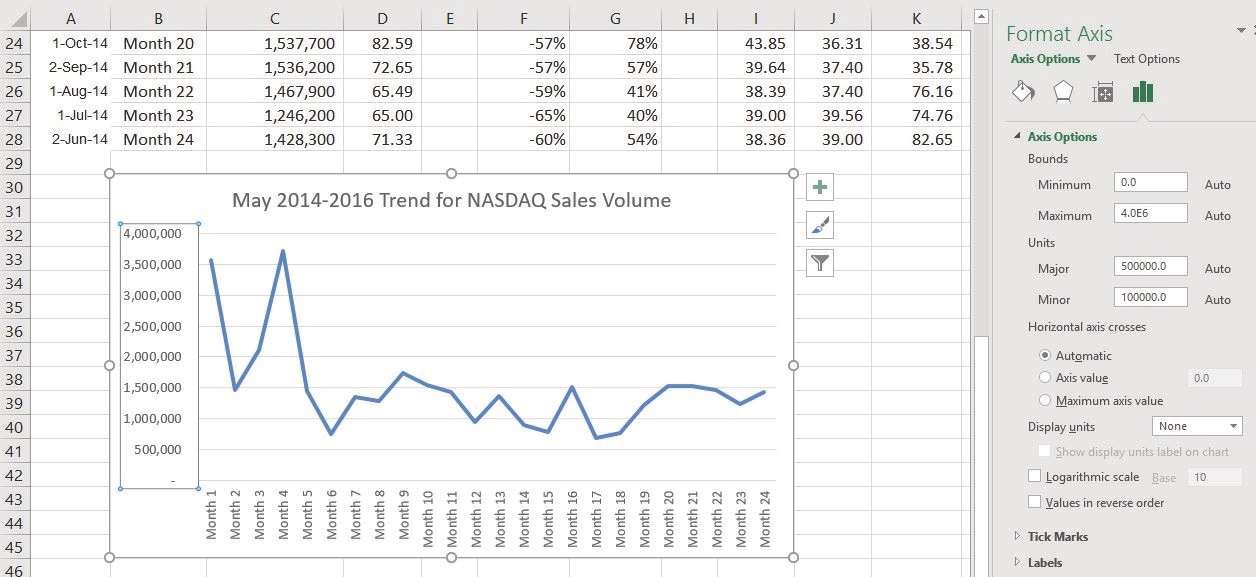
\includegraphics[width=\maxwidth{.95\linewidth}]{gfx/ch04_fig07}
	\caption{Trend Comparison Line Chart}
	\label{04:fig07}
\end{figure}

\begin{enumerate}
	\item Move the chart so the upper left corner is in the middle of cell \fmtCellLocation{M3}.
	\item Resize the chart, using the resizing handles and the \fmtKeystroke{Alt} key, so the left side is locked to the left side of Column M, the right side is locked to the right side of Column U, the top is locked to the top of Row $ 3 $, and the bottom is locked to the bottom of Row $ 17 $.
	\item Click in the text box that says \textit{Chart Title}. Delete the text and replace it with the following: \fmtTyping{24 Month Trend Comparison}.
\end{enumerate}

The Closing Price data is just a flat red line at the very bottom of the chart and cannot be seen very well. That is because the scale for this chart goes from $ 0 $ to $ 4,000,000 $ so the closing price data is compressed at the bottom of the scale. Complete the following steps to add a secondary axis to correct this problem.

\begin{enumerate}
	\item Right click the red line across the bottom of the chart that represents the \textit{Closing Price}.
	\item On the menu, select \fmtPopupButton{Format Data Series} to open the \fmtPopupBox{Format Data Series} pane.
	\item In the \fmtPopupBox{Series} Options, select \fmtPopupButton{Secondary Axis}.
\end{enumerate}

\begin{figure}[H]
	\centering
	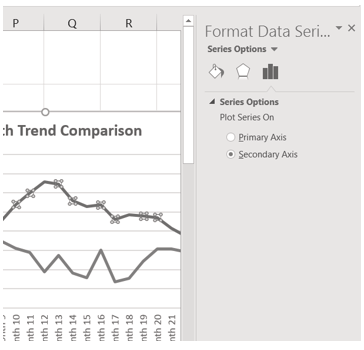
\includegraphics[width=\maxwidth{.95\linewidth}]{gfx/ch04_fig08}
	\caption{Adding a Secondary Axis}
	\label{04:fig08}
\end{figure}

The chart is better; but, it would be nice to be able to see that the values on the right represent prices rather than just numbers.

\begin{enumerate}
	\item Right click the Secondary Vertical Axis. (The vertical axis on the right that goes from $ 0 $ to $ 140 $.)
	\item From the menu, select \fmtPopupButton{Format Axis}.
	\item In \fmtPopupBox{Axis Options}, select \fmtPopupButton{Number}. (The menu may need to be scrolled down.)
	\item Use the \fmtPopupBox{Symbol} list box to add the \$.
	\item Press the \fmtPopupButton{Close} button to close the \fmtPopupBox{Format Axis} pane.
	\item Save the worksheet.
\end{enumerate}

\begin{figure}[H]
	\centering
	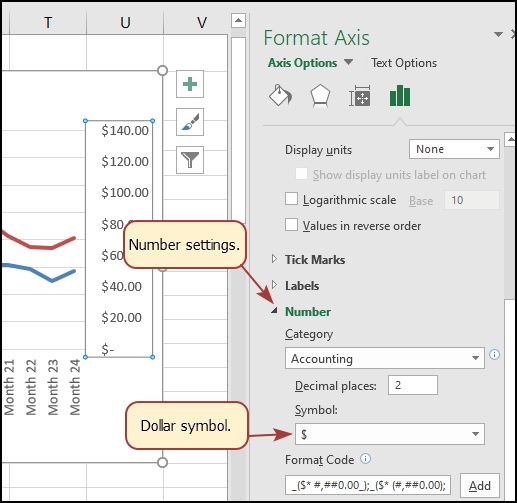
\includegraphics[width=\maxwidth{.95\linewidth}]{gfx/ch04_fig09}
	\caption{Modifying the Secondary Axis}
	\label{04:fig09}
\end{figure}

Now the chart makes it easy to compare the sales volume with the closing price.

\begin{figure}[H]
	\centering
	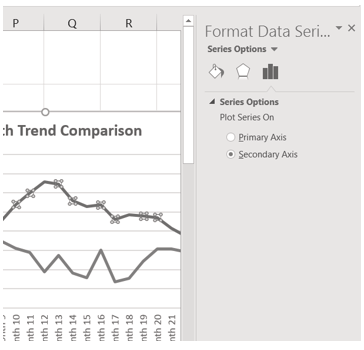
\includegraphics[width=\maxwidth{.95\linewidth}]{gfx/ch04_fig10}
	\caption{Final Comparison Line Chart}
	\label{04:fig10}
\end{figure}

\subsection{``Instant'' Chart – F11}

Excel includes an \fmtRibbonButton{Instant Chart} capability that makes charts easy to add with only a few mouse clicks. While these charts may need to be adjusted somewhat, they are often ready to use without any additional work. Follow these steps to add an ``instant'' chart.


\begin{enumerate}
	\item Select the \fmtWorksheetName{Stock Trend} worksheet.
	\item Select \fmtCellLocation{A4:A28}.
	\item Hold down the \fmtKeystroke{Ctrl} key and select \fmtCellLocation{D4:D28}. Figure \ref{04:fig11} shows what that will look like.
\end{enumerate}

\begin{figure}[H]
	\centering
	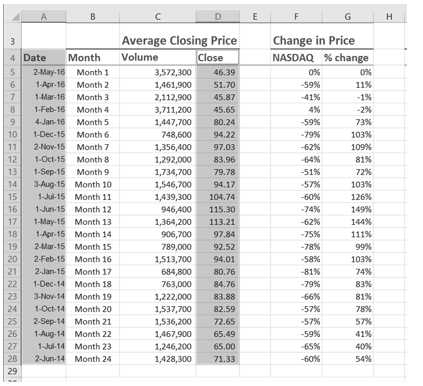
\includegraphics[width=\maxwidth{.95\linewidth}]{gfx/ch04_fig11}
	\caption{Range Selection}
	\label{04:fig11}
\end{figure}

\begin{enumerate}[resume]
	\item Press \fmtKeystroke{F11}. If the factory default settings have not been changed, Excel will create a column chart and place it on a separate chart sheet, as illustrated in Figure \ref{04:fig12}.
	\item Change the name of the chart sheet by double-clicking the worksheet name \textit{Chart1}. Type \fmtTyping{Closing Prices} as the new name and press \fmtKeystroke{Enter}.
	\item Save the worksheet.
\end{enumerate}

\begin{figure}[H]
	\centering
	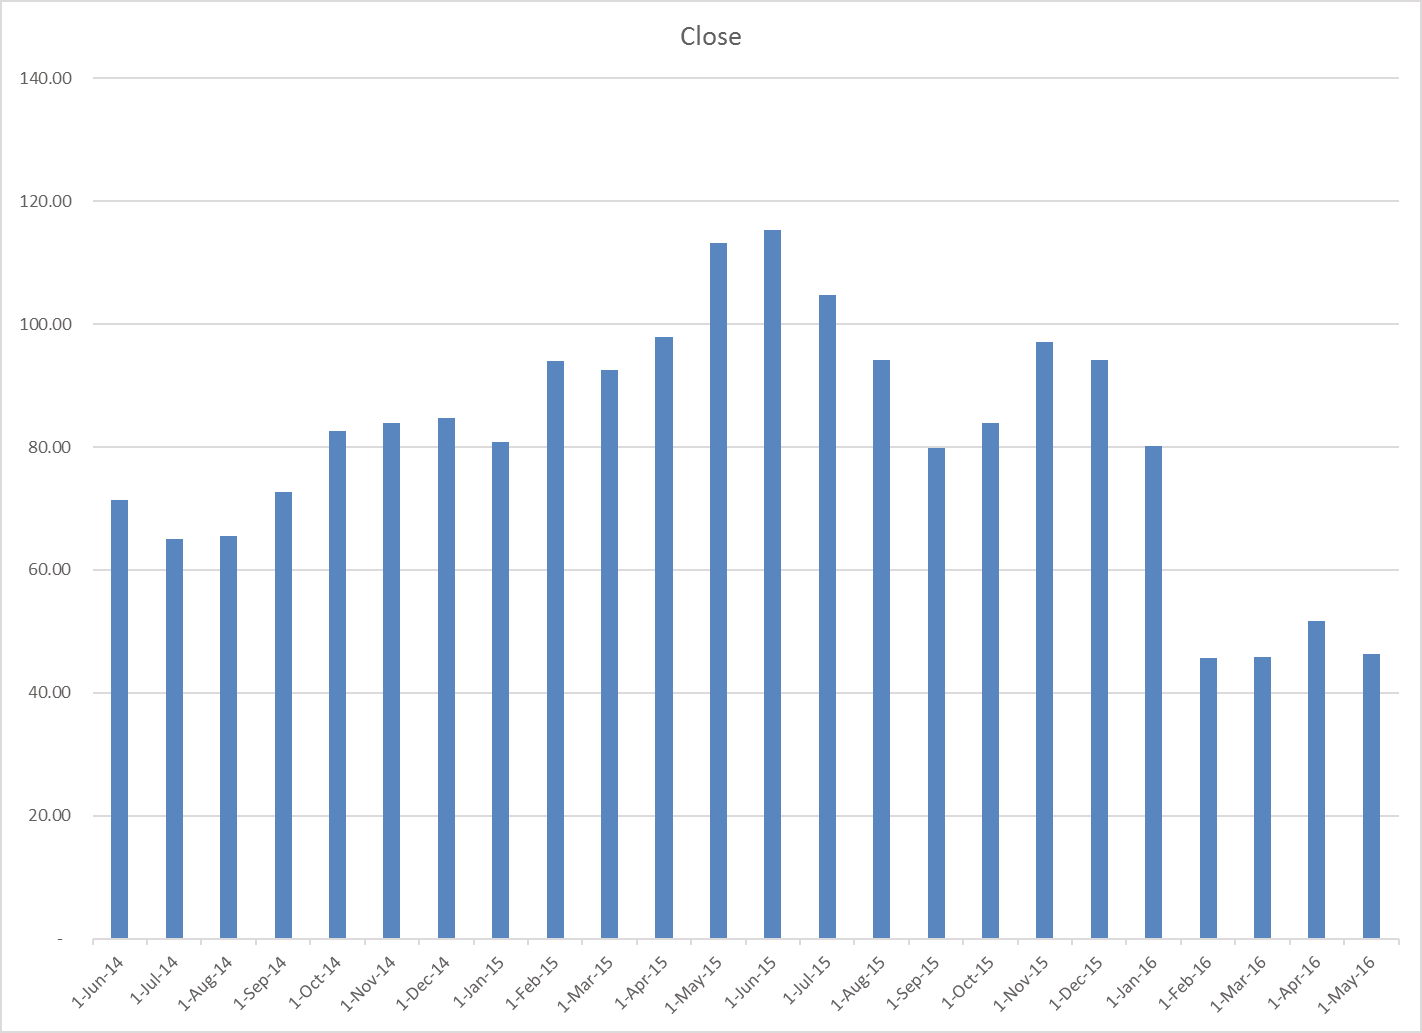
\includegraphics[width=\maxwidth{.95\linewidth}]{gfx/ch04_fig12}
	\caption{Instant Chart}
	\label{04:fig12}
\end{figure}

\subsection{Frequency Distribution: Column Chart 1}

A column chart is commonly used to show trends over time, as long as the data is limited to no more than twenty points. A common use for column charts is a frequency distribution, which shows the number of occurrences by established categories. For example, a common frequency distribution used in most academic institutions is a grade distribution. A grade distribution shows the number of students that achieve each level of a typical grading scale (A, A-, B+, B, etc.). The \fmtWorksheetName{Grade Distribution} worksheet contains final grades for several hypothetical Excel classes. To show the grade frequency distribution for all of the Excel classes in that year, the numbers of students appear on the Y axis and the grade categories appear on the X axis. The number of students for this chart is in Column C. The labels for grades are in Column A. The following steps explain how to create this chart.

\begin{enumerate}
	\item Select the \fmtWorksheetName{Grade Distribution} worksheet.
	\item Change the years in Row $ 3 $ to the current academic term and year.
	\item Highlight the range $ A3:A8 $ on the \fmtWorksheetName{Grade Distribution} worksheet. Column A shows the grade categories.
	\item Hold down the \fmtKeystroke{Crtl} key and select \fmtCellLocation{C3:C8}
	\item Click the \fmtRibbonButton{Column} button in the \fmtRibbonGroup{Charts} group section on the \fmtRibbonTab{Insert} tab of the ribbon. Select the first option in the 2-D Column section, which is the \fmtPopupBox{Clustered Column} format.
	\item Click and drag the chart so the upper left corner is in the middle of cell \fmtCellLocation{H2}.
	\item Resize the chart so the left side is locked to the left side of Column H, the right side is locked to the right side of Column O, the top is locked to the top of Row $ 2 $, and the bottom is locked to the bottom of Row $ 16 $.
	\item If Excel displays a legend, delete it by clicking the legend one time and pressing the \fmtKeystroke{Delete} key on the keyboard. Since the chart presents only one data series, the legend is not necessary.
	\item Add the text \fmtTyping{Final Grades} for to the chart title. The chart title should now be \fmtTyping{Final Grades for All Excel Classes 2020/2021} (or whichever academic year is being used).
	\item Click any cell location on the \fmtWorksheetName{Grade Distribution} worksheet to deactivate the chart.
	\item Save the worksheet.
\end{enumerate}

Figure \ref{04:fig13} shows the completed grade frequency distribution chart. By looking at the chart, it is obvious that the greatest number of students earned a final grade in the B+ to B- range.

\begin{figure}[H]
	\centering
	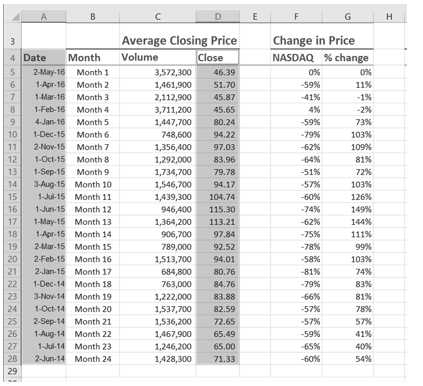
\includegraphics[width=\maxwidth{.95\linewidth}]{gfx/ch04_fig13}
	\caption{Grade Frequency Distribution Chart}
	\label{04:fig13}
\end{figure}

\subsection{Creating a Chart Sheet}

The charts that have been created up to this point have been added to, or embedded in, an existing worksheet (except the \fmtRibbonButton{Instant Chart} created using \fmtKeystroke{F11}). Charts can also be placed in a dedicated worksheet called a chart sheet. It is called a chart sheet because it can only contain an Excel chart. Chart sheets are useful to create several charts using the data in a single worksheet since it can be cumbersome to navigate and browse through multiple charts on a single worksheet. It is easier to browse through charts when they are moved to a chart sheet because a separate sheet tab is added to the workbook for each chart. The following steps explain how to move the grade frequency distribution chart to a dedicated chart sheet.

\begin{enumerate}
	\item Click anywhere on the \fmtPopupBox{Final Grades for All Excel Classes} chart on the \fmtWorksheetName{Grade Distribution} worksheet.
	\item Right click on the chart. Select \fmtPopupButton{Move Chart} This opens the \fmtPopupBox{Move Chart} Dialog box.
	\item Click the \fmtPopupButton{New sheet} option on the \fmtPopupBox{Move Chart} dialog box. (The top option.)
	\item The entry in the input box for assigning a name to the chart sheet tab should automatically be highlighted once the New sheet option is clicked. Type \fmtTyping{All Excel Classes}. This replaces the generic name in the input box (see Figure \ref{04:fig14}).
	\item Click the \fmtPopupButton{OK} button at the bottom of the \fmtPopupBox{Move Chart} dialog box. This adds a new chart sheet to the workbook with the name \fmtPopupBox{All Excel Classes}.
	\item Save the worksheet.
\end{enumerate}

\begin{figure}[H]
	\centering
	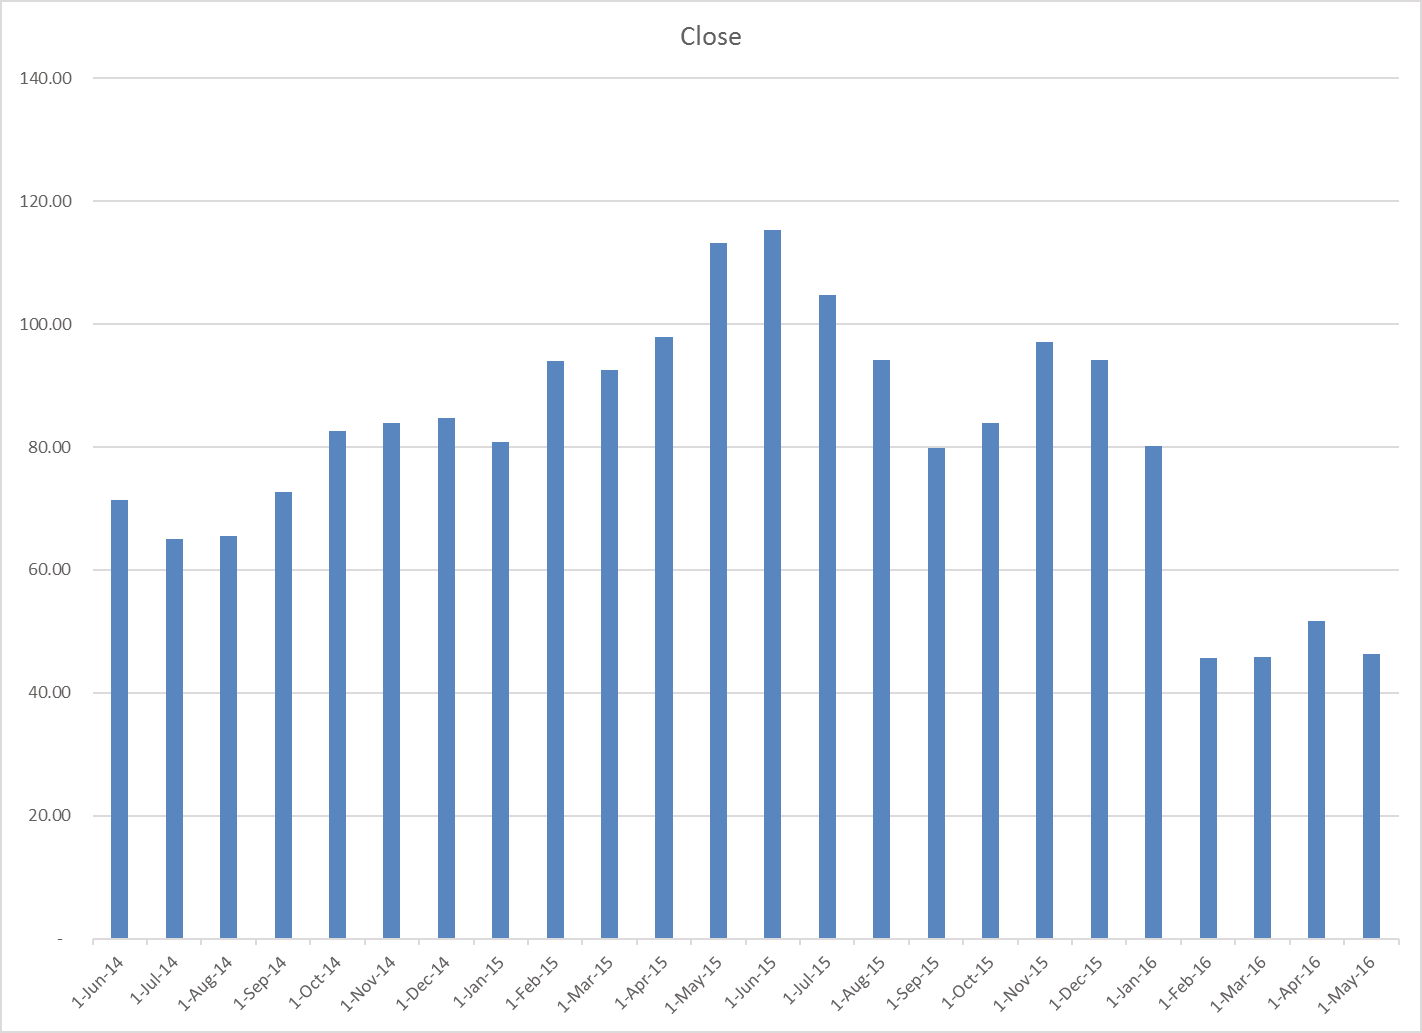
\includegraphics[width=\maxwidth{.95\linewidth}]{gfx/ch04_fig14}
	\caption{Moving a Chart to a Chart Sheet}
	\label{04:fig14}
\end{figure}

\begin{center}
	\begin{infobox}{Why?}
		\textbf{Column Chart vs. Bar Chart}
		\\
		\\
		When using charts to show frequency distributions, the difference between a column chart (where the bars are vertical) and a bar chart (where the bars are horizontal) is really a matter of preference. Both are very effective in showing frequency distributions. However, to show a trend over a period of time, a column chart is preferred over a bar chart. This is because a period of time is typically shown horizontally, with the oldest date on the far left and the newest date on the far right. Therefore, the descriptive categories for the chart would have to fall on the horizontal, or category, axis, which is the configuration of a column chart. On a bar chart, the descriptive categories are displayed on the vertical axis.
	\end{infobox}
\end{center}

Figure \ref{04:fig15} shows the \fmtPopupBox{Final Grades for all Excel Classes} column chart is in a separate chart sheet. Notice the new worksheet tab added to the workbook matches the name entered into the \fmtPopupBox{Move Chart} dialog box. Since the chart is moved to a separate chart sheet, it is no longer displayed in the \fmtWorksheetName{Grade Distribution} worksheet.

\begin{figure}[H]
	\centering
	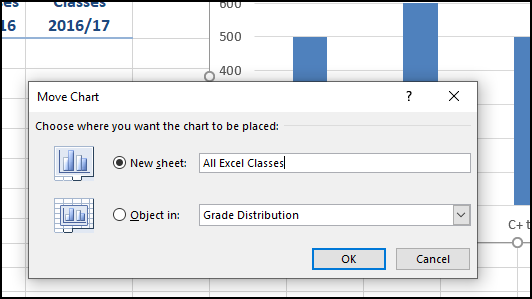
\includegraphics[width=\maxwidth{.95\linewidth}]{gfx/ch04_fig15}
	\caption{Chart Sheet Added to the Workbook}
	\label{04:fig15}
\end{figure}

\subsection{Frequency Comparison: Column Chart 2}

A second column chart will be created to show a comparison between two frequency distributions. Column B on the \fmtWorksheetName{Grade Distribution} worksheet contains data showing the number of students who received grades within each category for the Spring Quarter. This column chart will compare the grade distribution for Spring (Column B) with the overall grade distribution for the whole year (Column C). However, since the number of students in the term is significantly different from the total number of students in the year, a percentage must be calculated to make an effective comparison. The following steps explain how to calculate the percentages.

\begin{enumerate}
	\item Highlight the range \fmtCellLocation{B9:C9} on the \fmtWorksheetName{Grade Distribution} worksheet.
	\item Click the \fmtRibbonButton{AutoSum} button in the \fmtRibbonGroup{Editing} group of commands on the \fmtRibbonTab{Home} tab of the ribbon. This automatically adds \fmtPopupButton{SUM} functions that sum the values in the range \fmtCellLocation{B4:B8} and \fmtCellLocation{C4:C8}.
	\item Click in \fmtCellLocation{E4} on the \fmtWorksheetName{Grade Distribution} worksheet to activate that cell.
	\item Enter a formula that divides the value in cell \fmtCellLocation{B4} by the total in cell \fmtCellLocation{B9}. Add an absolute reference to cell \fmtCellLocation{B9} in the formula, like this \fmtTyping{=B4/\$B\$9}.
	\item Copy the formula in cell \fmtCellLocation{E4} and paste it into the range \fmtCellLocation{E5:E8} using the Paste command or with the Fill Handle.
	\item Activate cell \fmtCellLocation{F4} on the \fmtWorksheetName{Grade Distribution} worksheet.
	\item Enter a formula that divides the value in cell \fmtCellLocation{C4} by the total in cell \fmtCellLocation{C9}. Add an absolute reference to cell \fmtCellLocation{C9} in the formula, like this \fmtTyping{=C4/\$C\$9}.
	\item Copy the formula in cell \fmtCellLocation{F4} and paste it into the range \fmtCellLocation{F5:F8} using the Paste command or the Fill Handle.
\end{enumerate}

Figure \ref{04:fig16} shows the completed percentages added to the \fmtWorksheetName{Grade Distribution} worksheet.

\begin{figure}[H]
	\centering
	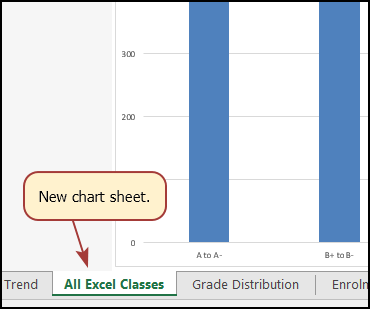
\includegraphics[width=\maxwidth{.95\linewidth}]{gfx/ch04_fig16}
	\caption{Completed Grade Distribution Percentages}
	\label{04:fig16}
\end{figure}

Next, create a column chart that uses the grade categories in the range \fmtCellLocation{A4:A8} on the X axis and the percentages in the range \fmtCellLocation{E4:F8} on the Y axis. 

\begin{enumerate}
	\item Select \fmtCellLocation{A3:A8} then hold down the \fmtKeystroke{Ctrl} key and select \fmtCellLocation{E3:F8}.
	\item Click the \fmtRibbonTab{Insert} tab of the ribbon.
	\item Click the \fmtRibbonButton{Column} button in the \fmtRibbonGroup{Charts} group of commands. Select the first option from the drop-down list of chart formats, which is the Clustered Column.
	\item Click and drag the chart so the upper left corner is in the middle of cell \fmtCellLocation{H2}.
	\item Resize the chart so the left side is locked to the left side of Column H, the right side is locked to the right side of Column N, the top is locked to the top of Row $ 2 $, and the bottom is locked to the bottom of Row $ 16 $.
	\item Change the chart title to \fmtTyping{Grade Distribution Comparison}. To add a chart title if one is not present, select \fmtRibbonButton{Add Chart Element} on the \fmtRibbonTab{Design} tab. Find the \fmtPopupBox{Chart Title} and select the \fmtPopupButton{Above Chart} option from the drop-down list.
	\item Save the workbook.
\end{enumerate}

Figure \ref{04:fig17} shows the completed data series operation.

\begin{figure}[H]
	\centering
	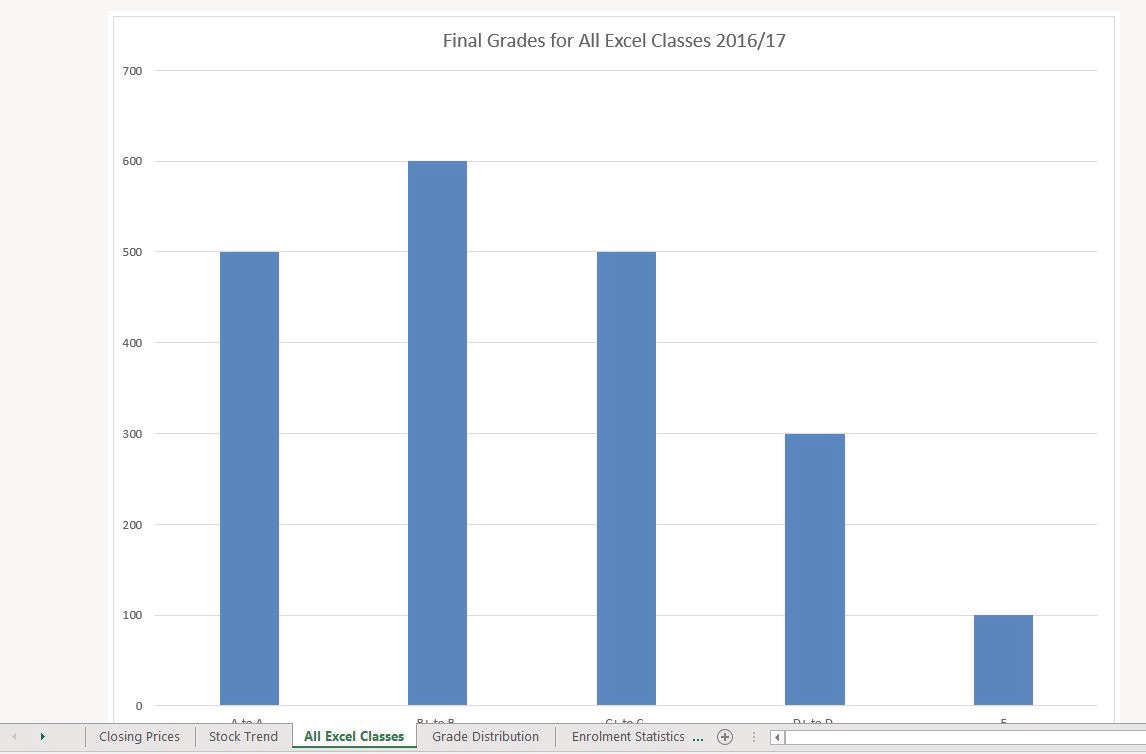
\includegraphics[width=\maxwidth{.95\linewidth}]{gfx/ch04_fig17}
	\caption{Completed Data Series for the Class Grade Distribution}
	\label{04:fig17}
\end{figure}

Figure \ref{04:fig18} shows the final appearance of the column chart. The column chart is an appropriate type for this data because there are fewer than twenty data points and it is easy to compare each category. A reader can quickly see that the class issued fewer \textit{As} compared to the rest of the college, but more \textit{Bs} and \textit{Cs}.

\begin{figure}[H]
	\centering
	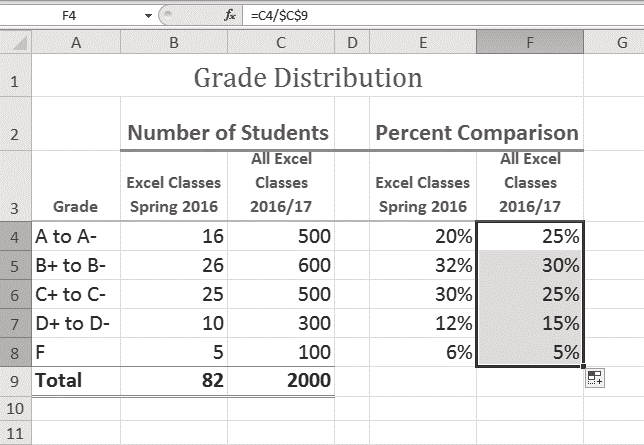
\includegraphics[width=\maxwidth{.95\linewidth}]{gfx/ch04_fig18}
	\caption{Completed Grade Distribution Column Chart}
	\label{04:fig18}
\end{figure}

\begin{center}
	\begin{infobox}{Integrity Check}
		\textbf{Too Many Bars on a Column Chart?}
		\\
		\\
		 Although there is no specific limit for the number of bars used on a column chart, a general rule of thumb is twenty bars or less. Figure \ref{04:fig19} contains a total of thirty-two bars. This is considered a poor use of a column chart because it is difficult to identify meaningful trends or comparisons. The data used to create this chart might be better used in two or three different column charts, each with a distinct idea or message.
	\end{infobox}
\end{center}

\begin{figure}[H]
	\centering
	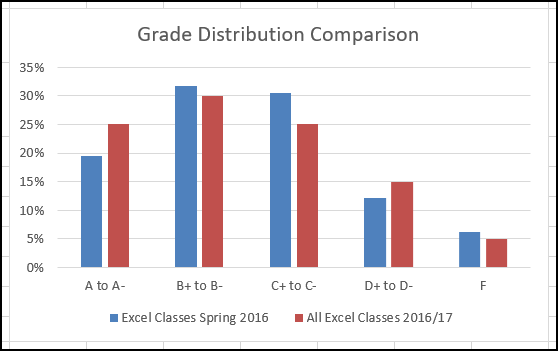
\includegraphics[width=\maxwidth{.95\linewidth}]{gfx/ch04_fig19}
	\caption{Poor Use of a Column Chart}
	\label{04:fig19}
\end{figure}

\subsection{Percent of Total: Pie Chart}

A pie chart is used to show a percent of total for a data set at a specific point in time. The data used to demonstrate a pie chart is related to enrollment data for Portland Area Community Colleges for Fall of 2014. That data is found on the \fmtWorksheetName{Enrollment Statistics} sheet.

\begin{enumerate}
	\item Highlight the range \fmtCellLocation{A2:B6} on the \fmtWorksheetName{Enrollment Statistics} worksheet.
	\item Click the \fmtRibbonTab{Insert} tab of the ribbon.
	\item Click the \fmtRibbonButton{Pie} button in the \fmtRibbonGroup{Charts} group of commands.
	\item Select the first 2-D Pie option from the drop-down list of options.
	\item To make the ``slices'' stand out better, choose to ``explode'' the pie chart.

	\begin{itemize}
		\item Click and hold the mouse button down in any of the slices of the pie. Note that there are selection handles on all of the pie slices.
		\item Without letting go of the mouse button, drag one of the slices away from the center.
		\item All of the slices ``explode'' out from the center.
	\end{itemize}

	\item Click off the slices and into the white canvas to deselect the pie and select the entire chart.
	\item Click and drag the pie chart so the upper left corner is in the middle of cell \fmtCellLocation{E2}.
	\item Resize the pie chart so the left side is locked to the left side of Column E, the right side is locked to the right side of Column L, the top is locked to the top of Row $ 2 $, and the bottom is locked to the bottom of Row $ 10 $ (see Figure \ref{04:fig20}).
\end{enumerate}

\textit{Note}: if the mouse button is released before dragging a ``slice'' of the pie then only one slice will move. This is another option for displaying the data. If this happens accidentally, use the \fmtRibbonButton{Undo} button to undo this and try again.

\begin{figure}[H]
	\centering
	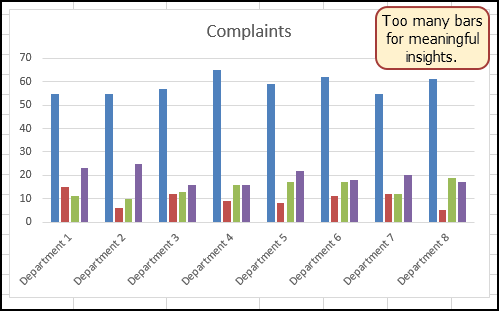
\includegraphics[width=\maxwidth{.95\linewidth}]{gfx/ch04_fig20}
	\caption{Pie Chart Moved and Resized}
	\label{04:fig20}
\end{figure}

\begin{enumerate}
	\item Click the chart legend once and press the \fmtKeystroke{Delete} key. A pie chart typically shows labels next to each slice. Therefore, the legend is not needed.
	\item Right click any of the slices in the pie chart, and select \fmtPopupButton{Add Data Labels} from the list. This will add the values for each of the slices in the pie.
	\item Now, right click one of the numbers and select \fmtPopupButton{Format Data Labels} from the list. This will open the \fmtPopupBox{Format Data Labels} pane on the right.
	\item Check the boxes for \fmtPopupButton{Category Name and Percentage} in the Label options section in the \fmtPopupBox{Format Data Labels} pane. This will add the Race/ethnicity labels as well as the percentage data to the pie chart.
	\item Uncheck the box next to the \fmtPopupButton{Value} box. This will remove the numbers from the pie chart (see Figure \ref{04:fig21}).
	\item Click the \fmtPopupButton{Close} button at the top of the \fmtPopupBox{Format Data Labels} pane.
	\item Select the data labels again (if needed). Click the \fmtRibbonTab{Home} tab of the ribbon and then click the \fmtRibbonButton{Bold} button. This will bold the data labels on the pie chart.
	\item Save the worksheet.
\end{enumerate}

\begin{figure}[H]
	\centering
	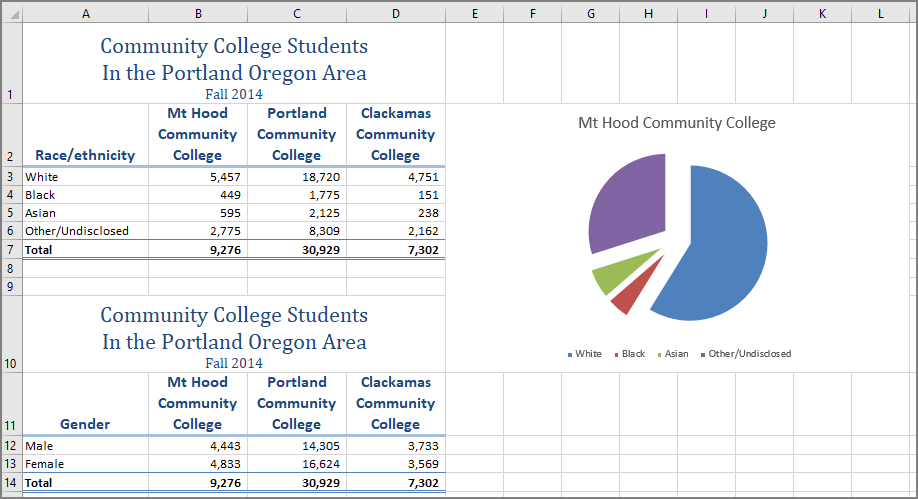
\includegraphics[width=\maxwidth{.95\linewidth}]{gfx/ch04_fig21}
	\caption{Final Settings in the Format Data Labels Pane}
	\label{04:fig21}
\end{figure}

Although there are no specific limits for the number of categories that can be used on a pie chart, a good rule of thumb is ten or less. As the number of  categories exceeds ten it becomes more difficult to identify key categories that make up the majority of the total. Figure \ref{04:fig22} shows the completed pie chart.

\begin{figure}[H]
	\centering
	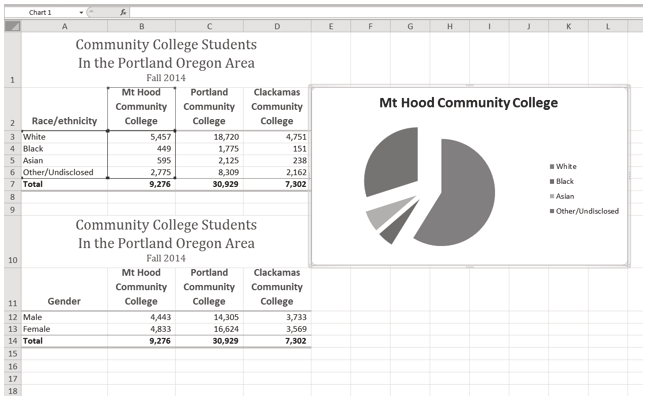
\includegraphics[width=\maxwidth{.95\linewidth}]{gfx/ch04_fig22}
	\caption{Final Enrollment Statistics Pie Chart}
	\label{04:fig22}
\end{figure}

\begin{center}
	\begin{sklbox}{Skill Refresher}
		\textbf{Inserting a Pie Chart}
		\\
		\begin{itemize}
			\setlength{\itemsep}{0pt}
			\setlength{\parskip}{0pt}
			\setlength{\parsep}{0pt}

			\item Highlight a range of cells that contain the data used to create the chart.
			\item Click the \fmtRibbonTab{Insert} tab of the ribbon.
			\item Click the \fmtRibbonButton{Pie} button in the \fmtRibbonGroup{Charts} group.
			\item Select a format option from the Pie Chart drop-down menu.
			
		\end{itemize}
	\end{sklbox}
\end{center}

\subsection{Percent of Total: Stacked Column Chart}

The last chart type demonstrated in this chapter is the stacked column chart. A stacked column chart is used  to show a percent of a total. For example, the data on the \fmtWorksheetName{Enrollment Statistics} worksheet shows student enrollment by race for several colleges. Suppose that it was necessary to show all of the data for all colleges.

\begin{enumerate}
	\item Highlight the range \fmtCellLocation{A2:D6} on the \fmtWorksheetName{Enrollment Statistics} worksheet.
	\item Click the \fmtRibbonTab{Insert} tab of the ribbon.
	\item Click the \fmtRibbonButton{Column} button in the \fmtRibbonGroup{Charts} group of commands. Select the \fmtPopupButton{100\% Stacked Column} format option from 2-D Column section in the drop-down list (see Figure \ref{04:fig23}).
\end{enumerate}

\begin{figure}[H]
	\centering
	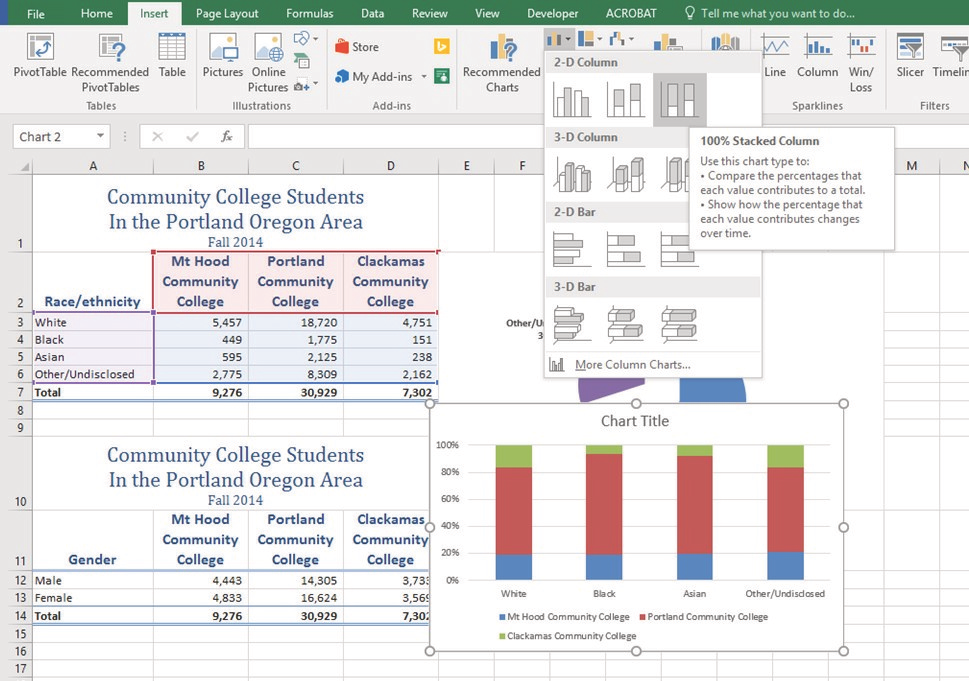
\includegraphics[width=\maxwidth{.95\linewidth}]{gfx/ch04_fig23}
	\caption{Selecting the 100\% Stacked Column Chart}
	\label{04:fig23}
\end{figure}

Figure \ref{04:fig24} shows the column chart that is created after selecting the \fmtPopupBox{100\% Stacked Column} format option. As mentioned, the goal of this chart is to show the enrollment of students by race. However, notice that Excel places the racial categories on the X axis. It would be more useful if the different colleges were there instead.

\begin{figure}[H]
	\centering
	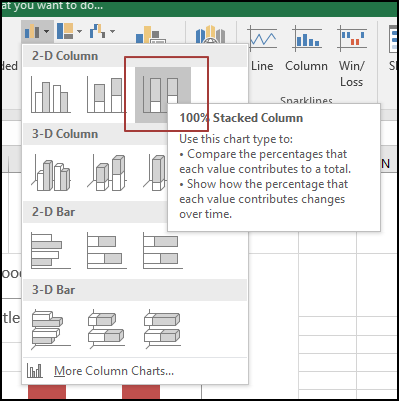
\includegraphics[width=\maxwidth{.95\linewidth}]{gfx/ch04_fig24}
	\caption{Initial Construction of the 100\% Stacked Column Chart}
	\label{04:fig24}
\end{figure}

The reason that Excel organized the data this way is that there are more Race/ethnicity categories (data in column A) than there are colleges (data in row 2). This is not a bad guess on Excel's part; but, this is not what is wanted in this case. The next steps explain how to correct this problem and complete the chart.

\begin{enumerate}
	\item Click the \fmtRibbonButton{Switch Row/Column} button in the \fmtRibbonTab{Design} tab on the \fmtRibbonGroup{Chart Tools} section of the ribbon. This reverses the legend and current X-Y axis categories.
\end{enumerate}

\begin{figure}[H]
	\centering
	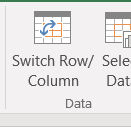
\includegraphics[width=\maxwidth{.95\linewidth}]{gfx/ch04_fig25}
	\caption{Switch Row/Column}
	\label{04:fig25}
\end{figure}

\begin{enumerate}[resume]
	\item Click and drag the chart so the upper left corner is in the middle of cell \fmtCellLocation{E12}.
	\item Resize the chart so the left side is locked to the left side of Column E, the right side is locked to the right side of Column N, the top is locked to the top of Row $ 12 $, and the bottom is locked to the bottom of Row $ 30 $.
	\item Click the legend one time and press the \fmtKeystroke{Delete} key on the keyboard.
	\item Add a Data Table. This is another way of displaying a legend for a column chart along with the numerical values that make up each component.

	\begin{itemize}
		\item In earlier versions of Excel, find the \fmtRibbonGroup{Labels} group of commands and select the \fmtRibbonButton{Show Data Table with Legend Keys} option from the drop-down menu.
		\item In Excel $ 2016 $, find the \fmtRibbonButton{Add Chart Element} tool on the \fmtRibbonTab{Design} tab, select \fmtRibbonButton{Data Table With Legend Keys}
	\end{itemize}

	\item Change the Chart Title to \fmtTyping{Enrollment by Race}. If there is no chart title, add one using the \fmtRibbonButton{Add Chart Element} tool on the \fmtRibbonTab{Design} tab.
	\item Save the worksheet.
\end{enumerate}

Figure \ref{04:fig26} shows the final stacked column chart. Notice the similarities and differences in the enrollment at the local community colleges.

\begin{figure}[H]
	\centering
	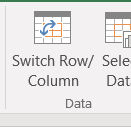
\includegraphics[width=\maxwidth{.95\linewidth}]{gfx/ch04_fig26}
	\caption{Final 100\% Stacked Column Chart}
	\label{04:fig26}
\end{figure}

\begin{center}
	\begin{sklbox}{Skill Refresher}
		\textbf{Inserting a Stacked Column Chart}
		\\
		\begin{itemize}
			\setlength{\itemsep}{0pt}
			\setlength{\parskip}{0pt}
			\setlength{\parsep}{0pt}

			\item Highlight a range of cells that contain data that will be used to create the chart.
			\item Click the \fmtRibbonTab{Insert} tab of the ribbon.
			\item Click the \fmtRibbonButton{Column} button in the \fmtRibbonGroup{Charts} group.
			\item Select the \fmtPopupButton{Stacked Column} format option from the \fmtPopupBox{Column Chart} drop-down menu to show the values of each category on the Y axis. Select the \fmtPopupButton{100\% Stacked Column} option to show the percent of total for each category on the Y axis.
			
		\end{itemize}
	\end{sklbox}
\end{center}

\begin{center}
	\begin{tkwbox}{Key Take-Aways}
		\textbf{Save}
		\\
		\begin{itemize}
			\setlength{\itemsep}{0pt}
			\setlength{\parskip}{0pt}
			\setlength{\parsep}{0pt}
			
			\item Identifying the message to be conveyed to an audience is a critical first step in creating an Excel chart.
			\item Both a column chart and a line chart can be used to present a trend over a period of time. However, a line chart is preferred over a column chart when presenting data over long periods of time.
			\item The number of bars on a column chart should be limited to twenty bars or less.
			\item When creating a chart to compare trends, the values for each data series must be within a reasonable range. If there is a wide variance between the values in the two data series (two times or more), the percent change should be calculated with respect to the first data point for each series.
			\item When working with frequency distributions, the use of a column chart or a bar chart is a matter of preference. However, a column chart is preferred when working with a trend over a period of time.
			\item A pie chart is used to present the percent of total for a data set.
			\item A stacked column chart is used to show how a percent total changes over time.

		\end{itemize}
	\end{tkwbox}
\end{center}

\section{Formatting Charts}

\begin{center}
	\begin{objbox}{Learning Objectives}
		\begin{itemize}
			\setlength{\itemsep}{0pt}
			\setlength{\parskip}{0pt}
			\setlength{\parsep}{0pt}

			\item Apply formatting commands to the X and Y axes.
			\item Enhance the visual appearance of the chart title and chart legend by using various formatting techniques.
			\item Assign titles to the X and Y axes that clarify labels and numeric values for the reader.
			\item Apply labels and formatting techniques to the data series in the plot area of a chart.
			\item Apply formatting commands to the chart area and the plot area of a chart.
			\item Employ series lines and annotations to enhance trends and provide additional information on a chart.
			
		\end{itemize}
	\end{objbox}
\end{center}

A variety of formatting techniques can be used to enhance the appearance of a chart once it is created. Formatting commands are applied to a chart for the same reason they are applied to a worksheet, they make the chart easier to read. However, formatting techniques also help qualify and explain the data in a chart. For example, footnotes can be added that explain the data source as well as notes that clarify the type of numbers being presented (\ie, if the numbers in a chart are truncated, a note can state whether they are in thousands, millions, etc.). These notes are also helpful in answering questions when using charts in a live presentation. This section demonstrates these formatting techniques using the column chart and stacked column chart from the previous section.

\subsection{X and Y Axis Formats}

There are numerous formatting commands that can be applied to the X and Y axes of a chart. Although adjusting the font size, style, and color are common, many more options are available through the Format Axis pane. The following steps demonstrate a few of these formatting techniques on the \fmtWorksheetName{Grade Distribution Comparison} chart.

\begin{enumerate}
	\item Switch to the \fmtWorksheetName{Grade Distribution} worksheet and click anywhere along the X axis (horizontal axis) of the \fmtPopupBox{Grade Distribution Comparison} chart.
	\item Right click and select \fmtPopupButton{Font}.
	\item Change the font to Arial, the Font Style to Bold, and the Size to $ 11 $ (see Figure \ref{04:fig27}).
\end{enumerate}

\begin{figure}[H]
	\centering
	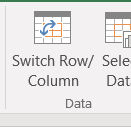
\includegraphics[width=\maxwidth{.95\linewidth}]{gfx/ch04_fig27}
	\caption{Font Dialog Box}
	\label{04:fig27}
\end{figure}

\begin{enumerate}[resume]
	\item Click anywhere along the Y axis to activate it and repeat steps $ 2 $ and $ 3 $.
	\item Click on the chart title and repeat steps $ 2 $ and $ 3 $, but set the Size to $ 14 $.
	\item The final appearance of the axes is shown in Figure \ref{04:fig28}.
\end{enumerate}

\begin{figure}[H]
	\centering
	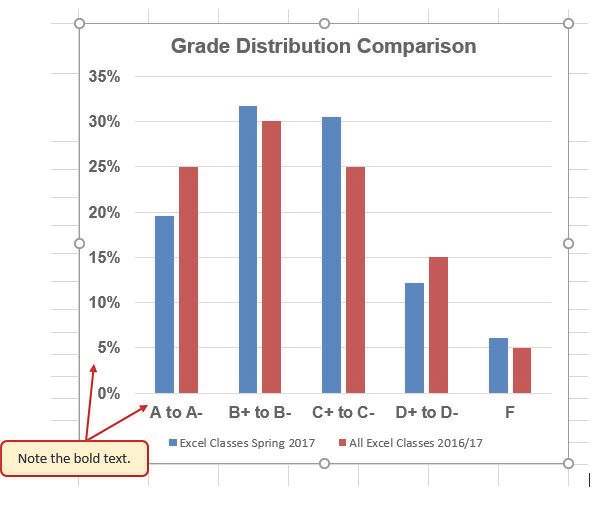
\includegraphics[width=\maxwidth{.95\linewidth}]{gfx/ch04_fig28}
	\caption{Formatted X and Y Axes}
	\label{04:fig28}
\end{figure}

Next, make some changes to the percentage numbers on the Y (vertical) axis.

\begin{enumerate}
	\item Right click the vertical (value) axis. Select \fmtPopupButton{Format Axis}. This opens the \fmtPopupBox{Format Axis} pane.
	\item Click \fmtPopupButton{Number} from the list of options. The commands in this section of the \fmtPopupBox{Format Axis} pane are used to format numbers that appear on the selected axis of the chart.
	\item Click in the \fmtPopupBox{Decimal} places input box and change the value to $ 1 $.
	\item Select \fmtPopupButton{Axis Options}. Change the \fmtPopupBox{Minimum Bound} to $ .05 $ to make the differences in the columns more dramatic. The \fmtPopupBox{Format Axis} pane should match Figure \ref{04:fig29}.
	\item Click the \fmtPopupButton{Close} button at the top of the \fmtPopupBox{Format Axis} pane.
	\item Save the workbook.
\end{enumerate}

\begin{figure}[H]
	\centering
	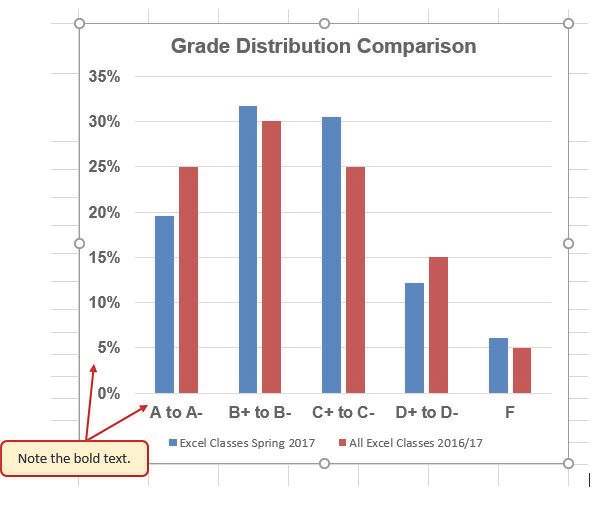
\includegraphics[width=\maxwidth{.95\linewidth}]{gfx/ch04_fig29}
	\caption{Format Axis Pane Changes}
	\label{04:fig29}
\end{figure}

\begin{center}
	\begin{infobox}{Note}
		\textbf{Experiment!}
		\\
		\\
		The font styling can also be changed using shortcut keys and the buttons on the \fmtRibbonTab{Home} tab.
	\end{infobox}
\end{center}

\begin{center}
	\begin{sklbox}{Skill Refresher}
		\textbf{Formatting the X and Y Axes}
		\\
		\begin{itemize}
			\setlength{\itemsep}{0pt}
			\setlength{\parskip}{0pt}
			\setlength{\parsep}{0pt}

			\item Click anywhere along the X or Y axis to activate it.
			\item Click either the \fmtRibbonTab{Home} tab or \fmtRibbonTab{Design} tab of the ribbon.
			\item Select any of the available formatting commands in these tabs.
			
		\end{itemize}
	\end{sklbox}
\end{center}

\begin{center}
	\begin{sklbox}{Skill Refresher}
		\textbf{X and Y Axis Number Formats}
		\\
		\begin{itemize}
			\setlength{\itemsep}{0pt}
			\setlength{\parskip}{0pt}
			\setlength{\parsep}{0pt}

			\item Click anywhere along the X or Y axis to activate it.
			\item Click the \fmtRibbonTab{Layout} tab in the \fmtRibbonGroup{Chart Tools} section of the ribbon.
			\item Click the \fmtRibbonButton{Format Selection} button in the \fmtRibbonGroup{Current Selection} group of commands.
			\item Click \fmtPopupButton{Number} from the list of options on the left side of the \fmtPopupBox{Format Axis} dialog box.
			\item Select a number format and set decimal places on the right side of the \fmtPopupBox{Format Axis} dialog box.
			\item Click the \fmtPopupButton{Close} button in the \fmtPopupBox{Format Axis} pane.
			
		\end{itemize}
	\end{sklbox}
\end{center}

\subsection{Chart Legend and Title Formats}

The next items to be formatted on the \fmtPopupBox{Grade Distribution Comparison} chart are the chart legend and title. Similar to the X and Y axes, format these items by activating them and using commands in the \fmtRibbonTab{Home} tab or the \fmtPopupBox{Format} pane. The following steps explain how to change these formats.

\begin{enumerate}
	\item Right click the legend on the \fmtPopupBox{Grade Distribution Comparison} chart and select \fmtPopupButton{Format Legend}.
	\item Select \fmtPopupButton{Right} in the \fmtPopupBox{Legend Position} options. Close the \fmtPopupBox{Format Legend} pane.
	\item Move the legend by placing the cursor, shaped like a little plus sign with four arrows, on the edge of the selection box. Click and drag the legend so the top of the legend aligns with the $ 35\% $ line next to the plot area (see Figure \ref{04:fig30}).
\end{enumerate}

\begin{figure}[H]
	\centering
	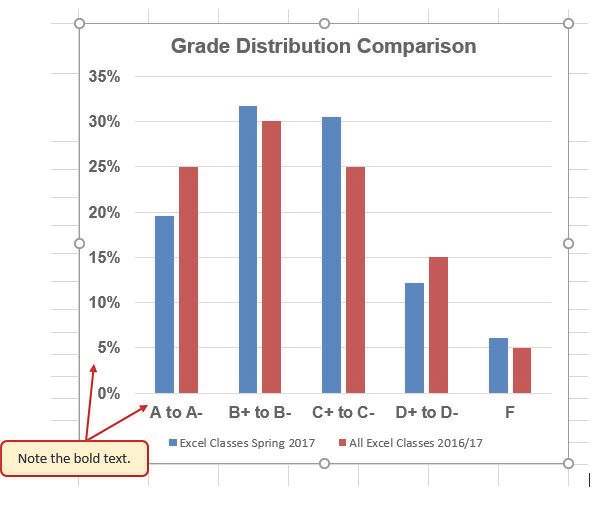
\includegraphics[width=\maxwidth{.95\linewidth}]{gfx/ch04_fig30}
	\caption{Moving the Legend}
	\label{04:fig30}
\end{figure}

\begin{enumerate}
	\item While the legend is still selected, change the font style in the \fmtRibbonTab{Home} tab of the ribbon to Arial.
	\item Change the font size to $ 12 $ points.
	\item Click the bold and italics commands in the \fmtRibbonTab{Home} tab of the ribbon.
	\item Click and drag the left sizing handle so the legend is against the plot area (see Figure \ref{04:fig31}).
\end{enumerate}

\begin{figure}[H]
	\centering
	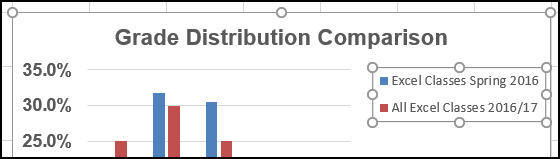
\includegraphics[width=\maxwidth{.95\linewidth}]{gfx/ch04_fig31}
	\caption{Legend Formatted and Resized}
	\label{04:fig31}
\end{figure}

\begin{enumerate}
	\item Click the chart title to activate it.
	\item Right click on the chart title and select \fmtPopupButton{Format Chart Title} to open the \fmtPopupBox{Format Chart Title} pane (see Figure \ref{04:fig32}).
	\item Under \fmtPopupBox{Title Options} in the Effects group (the option in the middle) give the title one of the Preset shadows. Also, change the color if desired.
	\item Close the \fmtPopupBox{Format Chart Title} pane.
	\item Save the workbook.
\end{enumerate}

\begin{figure}[H]
	\centering
	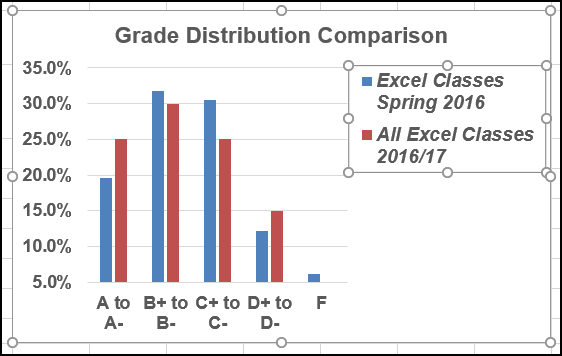
\includegraphics[width=\maxwidth{.95\linewidth}]{gfx/ch04_fig32}
	\caption{Format Chart Title Pane}
	\label{04:fig32}
\end{figure}

\begin{center}
	\begin{sklbox}{Skill Refresher}
		\textbf{Formatting the Chart Legend}
		\\
		\begin{itemize}
			\setlength{\itemsep}{0pt}
			\setlength{\parskip}{0pt}
			\setlength{\parsep}{0pt}

			\item Click the Legend to activate it.
			\item Click either the \fmtRibbonTab{Home} tab or right click to activate the appropriate formatting pane.
			\item Select any of the available formatting commands.
			\item Click and drag the legend to move it.
			\item Click and drag any of the sizing handles to adjust the size of the legend.
			
		\end{itemize}
	\end{sklbox}
\end{center}

\begin{center}
	\begin{sklbox}{Skill Refresher}
		\textbf{Formatting the Chart Title}
		\\
		\begin{itemize}
			\setlength{\itemsep}{0pt}
			\setlength{\parskip}{0pt}
			\setlength{\parsep}{0pt}

			\item Click anywhere on the chart title.
			\item Click either the \fmtRibbonTab{Home} tab or right click to activate the appropriate formatting pane.
			\item Select any of the available formatting commands.
			
		\end{itemize}
	\end{sklbox}
\end{center}

\subsection{X and Y Axis Titles}

Titles for the X and Y axes are necessary for defining the numbers and categories presented on a chart. For example, by looking at the \fmtPopupBox{Grade Distribution Comparison} chart, it is not clear what the percentages along the Y axis represent. The following steps explain how to add titles to the X and Y axes to define these numbers and categories.

\begin{enumerate}
	\item Click anywhere on the \fmtPopupBox{Grade Distribution Comparison} chart in the \fmtWorksheetName{Grade Distribution} worksheet to activate it.
	\item On the \fmtRibbonTab{Design} tab on the ribbon select the \fmtRibbonButton{Add Chart Element} button, then \fmtRibbonButton{Axis Titles}, then \fmtRibbonButton{Primary Vertical}. (See Figure \ref{04:fig33})
\end{enumerate}

\begin{figure}[H]
	\centering
	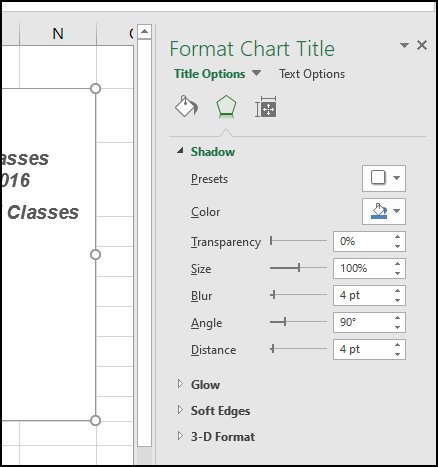
\includegraphics[width=\maxwidth{.95\linewidth}]{gfx/ch04_fig33}
	\caption{Selecting a Title for the Y Axis}
	\label{04:fig33}
\end{figure}

\begin{enumerate}
	\item Using the \fmtRibbonTab{Home} ribbon, change the font of the axis title to Arial, Bold, size $ 11 $.
	\item Click in the beginning of the Y axis title and delete the generic title. Type \fmtTyping{Percent of Enrolled Excel Students}.(see Figure \ref{04:fig34}).
\end{enumerate}

\begin{figure}[H]
	\centering
	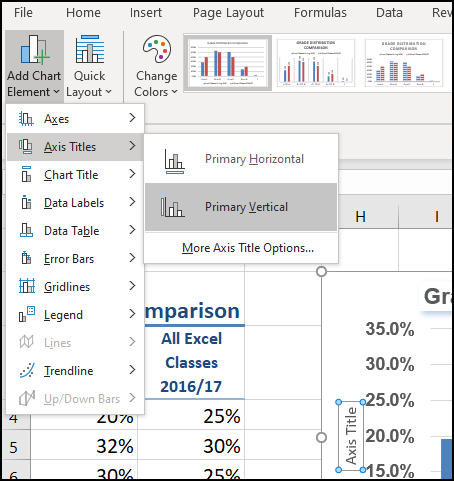
\includegraphics[width=\maxwidth{.95\linewidth}]{gfx/ch04_fig34}
	\caption{Adding and Formatting the Y Axis Title}
	\label{04:fig34}
\end{figure}

Next, add the title for the X axis.

\begin{enumerate}
	\item On the \fmtRibbonTab{Design} tab select the \fmtRibbonButton{Add Chart Element} button, then \fmtRibbonButton{Axis Titles}, then \fmtRibbonButton{Primary Horizontal}.
	\item Using the \fmtRibbonTab{Home} ribbon, change the font of the axis title to Arial, Bold, size $ 11 $. 
	\item Click in the beginning of the X axis title and delete the generic title. Type \fmtTyping{Final Course Grade}. Figure \ref{04:fig35} shows the added titles for the X and Y axes. The titles provide definitions for the grade categories along the X axis as well as the percentages on the Y axis.
	\item Save the workbook.
\end{enumerate}

\begin{figure}[H]
	\centering
	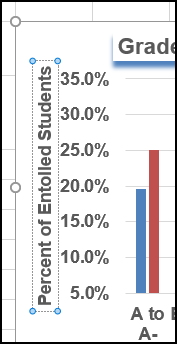
\includegraphics[width=\maxwidth{.95\linewidth}]{gfx/ch04_fig35}
	\caption{X and Y Axis Titles Added}
	\label{04:fig35}
\end{figure}

\begin{center}
	\begin{sklbox}{Skill Refresher}
		\textbf{X and Y Axis Titles}
		\\
		\begin{itemize}
			\setlength{\itemsep}{0pt}
			\setlength{\parskip}{0pt}
			\setlength{\parsep}{0pt}

			\item On the \fmtRibbonTab{Design} tab select the \fmtRibbonButton{Add Chart Element} button.
			\item Click anywhere on the chart to activate it.
			\item Select one of the options from the second drop-down list.
			\item Click in the axis title to remove the generic title and type a new title.
			
		\end{itemize}
	\end{sklbox}
\end{center}

\subsection{Data Series Labels and Formats}

Adding labels to the data series of a chart is a key formatting feature. A data series is the item that is being displayed graphically on a chart. For example, the blue bars on the Grade Distribution

Comparison charts represent one data series. Labels can be added at the end of each bar to show the exact percentage the bar represents. In addition, other formatting enhancements can be added to the data series, such as changing the color of the bars or adding an effect. The following steps explain how to add these labels and formats to the chart.

\begin{enumerate}
	\item Click on any of the the red bars representing the \fmtPopupBox{All Excel Classes} data series on the \fmtPopupBox{Grade Distribution Comparison} chart in the \fmtWorksheetName{Grade Distribution} worksheet. Clicking one bar automatically activates all bars in the data series. If a bar is clicked a second time, only that one bar is activated.
	\item Right click and select \fmtPopupButton{Format Data Series} to open up the \fmtPopupBox{Format Data Series} pane.
	\item Click the \fmtPopupButton{Fill and Line} (paint bucket) button to bring up the \fmtPopupBox{Fill and Border} group of commands.
	\item Click the word \fmtPopupButton{Fill} (if needed) to expand the list of Fill options.
	\item Select \fmtPopupButton{Pattern Fill}. Then select $ 30\% $ (fifth column, top row). Changing the fill pattern to a pattern makes it easier to distinguish between the data series when the chart is printed or viewed in black and white. Experiment with the fill pattern by selecting different foreground and background colors.
	\item Close the \fmtPopupBox{Format Data Series} pane.
\end{enumerate}

\begin{figure}[H]
	\centering
	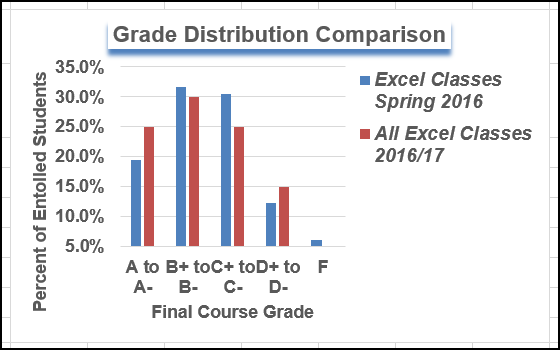
\includegraphics[width=\maxwidth{.95\linewidth}]{gfx/ch04_fig36}
	\caption{Changing the Fill of a Data Series}
	\label{04:fig36}
\end{figure}

Next, add the Data Labels at the end of the columns.

\begin{enumerate}
	\item Be sure that the entire chart is selected, not just one of the data series. Click the \fmtRibbonTab{Design} tab in the \fmtRibbonGroup{Chart Tools} section of the ribbon.
	\item On the \fmtRibbonTab{Design} tab select the \fmtRibbonButton{Add Chart Element} button, then \fmtRibbonButton{Data Labels}, then \fmtRibbonButton{Outside End} (see Figure \ref{04:fig37}.)
	\item Click on one of the Data Labels. Note that all of the data labels for that data series are selected.
	\item Using the \fmtRibbonTab{Home} ribbon, change the font to Arial, Bold, size $ 9 $.
	\item Click on one of the data labels for the other data series. Format those data labels as Arial, Bold, size $ 9 $ as well.
	\item Save the workbook.
\end{enumerate}

\begin{figure}[H]
	\centering
	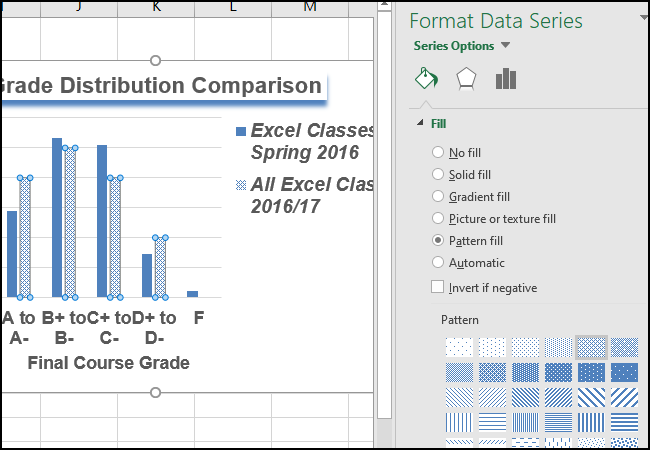
\includegraphics[width=\maxwidth{.95\linewidth}]{gfx/ch04_fig37}
	\caption{Adding Labels to a Data Series}
	\label{04:fig37}
\end{figure}

Figure \ref{04:fig38} shows the \fmtPopupBox{Grade Distribution Comparison} chart with the completed formatting adjustments and labels added to the data series. Note that each individual data label can be moved if two data labels overlap or if a data label falls in the middle of a grid line. To move an individual data label, click it twice and then click and drag.

\begin{figure}[H]
	\centering
	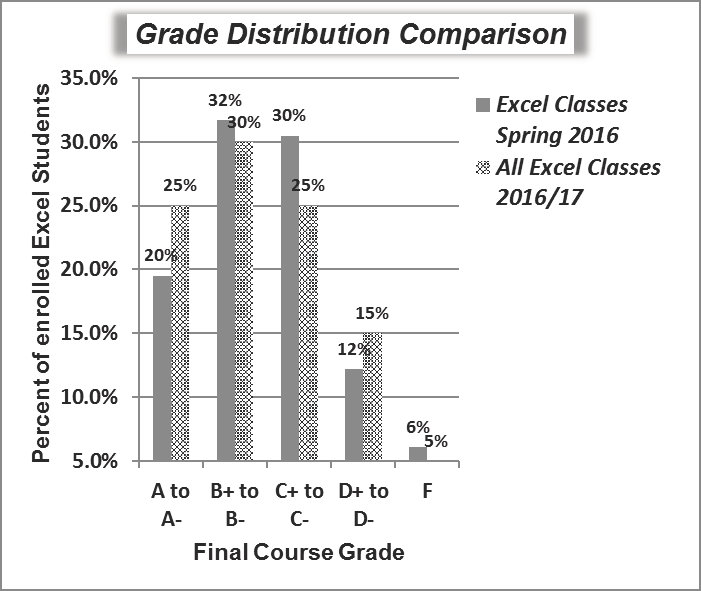
\includegraphics[width=\maxwidth{.95\linewidth}]{gfx/ch04_fig38}
	\caption{Completed Formatting Adjustments for the Data Series}
	\label{04:fig38}
\end{figure}

\begin{center}
	\begin{sklbox}{Skill Refresher}
		\textbf{Adding Data Labels}
		\\
		\begin{itemize}
			\setlength{\itemsep}{0pt}
			\setlength{\parskip}{0pt}
			\setlength{\parsep}{0pt}

			\item Click anywhere on the chart to activate it.
			\item Click the \fmtRibbonTab{Design} tab in the \fmtRibbonGroup{Chart Tools} section of the ribbon.
			\item Click the \fmtRibbonButton{Add Chart Element} in the \fmtRibbonGroup{Chart Layout} group.
			\item Select \fmtRibbonButton{Data Labels}
			\item Select one of the preset positions from the drop-down list.
			
		\end{itemize}
	\end{sklbox}
\end{center}

\begin{center}
	\begin{sklbox}{Skill Refresher}
		\textbf{Formatting a Data Series}
		\\
		\begin{itemize}
			\setlength{\itemsep}{0pt}
			\setlength{\parskip}{0pt}
			\setlength{\parsep}{0pt}
			
			\item Click any bar or line for a data series.
			\item Right click to activate the \fmtPopupBox{Format Data Series} pane.
			\item Use the formatting tools in the pane to make changes to the data series.
			
		\end{itemize}
	\end{sklbox}
\end{center}

\subsection{Adding Series Lines and Annotations to a Chart}

The last formatting features demonstrated are adding series lines and annotations to a chart. To demonstrate these skills, use the \fmtPopupBox{Change in Enrollment Statistics Spend Source} stacked column chart. Series lines are commonly used in stacked column charts to show the change from one stack to the next. Annotations are useful for clarifying the data presented in a chart or for identifying data sources. In addition to demonstrating these skills, this section will review several of the formatting skills that were covered earlier. The following steps include the skills review as well as the new formatting features.

\begin{enumerate}
	\item Locate the \fmtPopupBox{Enrollment by Race} stacked column chart on the \fmtWorksheetName{Enrollment Statistics} worksheet. Activate the chart by clicking anywhere inside the chart perimeter.
	\item Move the chart to a separate chart sheet by clicking the \fmtRibbonButton{Move Chart} button in the \fmtRibbonTab{Design} tab of the ribbon. Type the following in the New sheet input box: \fmtTyping{Enrollment by Race Chart}. Click the \fmtPopupButton{OK} button.
	\item Click anywhere on the data table (on the x axis) to activate it. Using the \fmtRibbonTab{Home} ribbon, change the font to Arial, Bold, size $ 12 $.
	\item Activate the Y axis and apply the same formatting adjustments as stated in step $ 3 $. 
	\item Add a Y axis title using \fmtRibbonButton{Add Chart Elements} then \fmtRibbonButton{Axis Titles} then \fmtRibbonButton{More Axis Title Options}.
	\item In the \fmtPopupBox{Format Axis Title} pane change the fill color and border to any colors desired.
	\item Then, using the \fmtRibbonTab{Home} tab of the ribbon, change the font to Arial, Bold, size $ 14 $.
	\item Change the text of the Y axis title to \fmtTyping{Percent Enrollment by Race}.
	\item Check the horizontal axis to see if this process created an extra axis title there. If it did, delete it.
	\item Activate the title of the chart by clicking it once. The \fmtPopupBox{Format Chart Title} pane should be open. If not, right click the Chart title and select \fmtPopupButton{Format Chart Title} from the menu. Change the fill and border to match the vertical Axis label.
	\item Then, using the \fmtRibbonTab{Home} tab of the ribbon, change the font of the chart title to Arial, Bold, size $ 20 $.
	\item Close the \fmtPopupBox{Formatting} pane.
	\item Click the \fmtRibbonButton{Add Chart Elements} tool (\fmtRibbonTab{Design} tab), then \fmtRibbonButton{Lines}, then \fmtRibbonButton{Series Lines}. This adds lines to the chart, connecting each data series between the three stacks (see Figure \ref{04:fig39}).
\end{enumerate}

\begin{figure}[H]
	\centering
	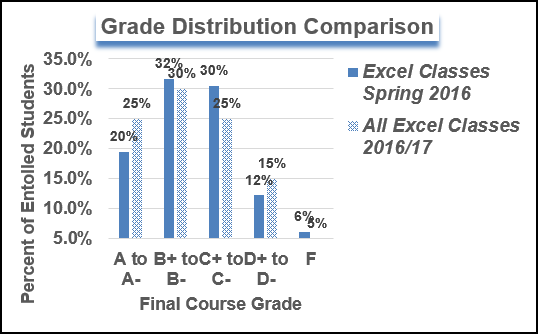
\includegraphics[width=\maxwidth{.95\linewidth}]{gfx/ch04_fig39}
	\caption{Selecting the Series Lines Option}
	\label{04:fig39}
\end{figure}

\begin{enumerate}
	\item Right click on any of the series lines added to the chart. Clicking one line will activate all lines on the chart. (If the \fmtPopupBox{Format} pane is open there is no need to right click. Just left click on any of the series lines to change the format pane to \fmtPopupBox{Format Series Lines}.)
	\item Select \fmtPopupButton{Format Series Lines}. This will open the \fmtPopupBox{Format Series Lines} pane.
	\item Change the width to $ 2.25 $.
	\item Close the \fmtPopupBox{Format Series Lines} pane.
\end{enumerate}

Figure \ref{04:fig40} shows the appearance of the chart with the series lines connecting the two stacks. This formatting enhancement is common for stacked column charts. The lines help focus the audience's attention to changes in the percent of total trend.

\begin{figure}[H]
	\centering
	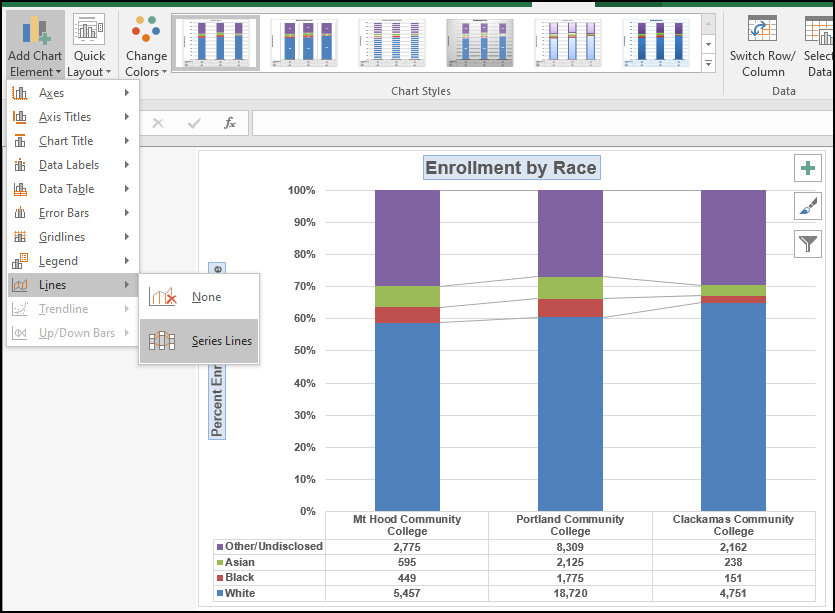
\includegraphics[width=\maxwidth{.95\linewidth}]{gfx/ch04_fig40}
	\caption{Series Lines Added to the Stacked Column Chart}
	\label{04:fig40}
\end{figure}

The chart demonstrates the percentage differences in enrollment between the community colleges. But, it would be handy to know the total enrollment at each of the colleges. To display that, add text boxes above each column. To start, make room for the text boxes.

\begin{enumerate}
	\item Select the Plot Area. Place cursor on the top center handle of the Plot Area and drag down about $ 1/2 $ inch. (See Figure \ref{04:fig41}.)
\end{enumerate}

\begin{figure}[H]
	\centering
	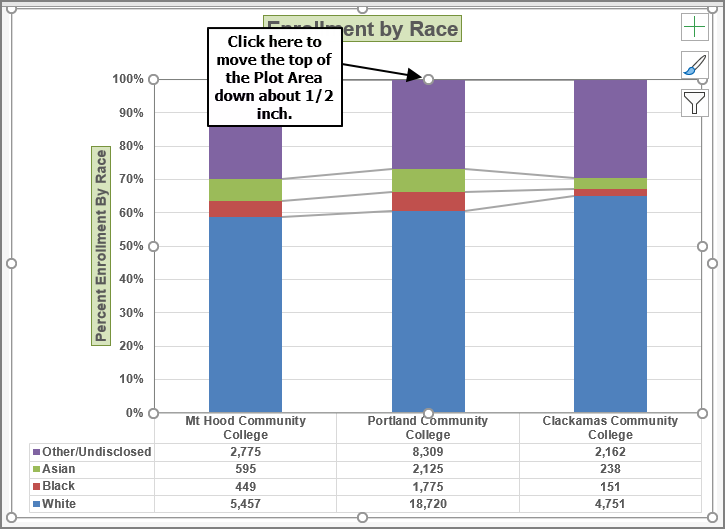
\includegraphics[width=\maxwidth{.95\linewidth}]{gfx/ch04_fig41}
	\caption{Resizing the Plot Area}
	\label{04:fig41}
\end{figure}

\subsection{Add Text Boxes to Include Additional Information in the Chart.}

\begin{enumerate}
	\item Click the \fmtRibbonButton{Text Box} button in the \fmtRibbonGroup{Text} group on the \fmtRibbonTab{Insert} tab of the ribbon (see Figure \ref{04:fig42}). 
	\item Place the mouse pointer on the left edge of the chart area approximately one-quarter inch from the top. Click and drag a rectangle approximately one and a half inches wide and one-quarter inch high (see Figure \ref{04:fig42}). Do not worry if it is not exact, it can be moved and resized at any time.
	\item Type \fmtTyping{Total Enrollment}. This tells the audience the size of each school.
	\item Select all of the text in the text box. (The text can be selected by either dragging over it with the mouse or by clicking on the border of the text box once). Using the \fmtRibbonTab{Home} tab of the ribbon, change the font to Arial, size $ 14 $.
	\item Repeat the process to add and format text boxes above each column. The boxes can be copy/pasted to save time.
	\item In each text box, type the Total Enrollment for each school:

	\begin{itemize}
		\item Mt Hood --- 9,276
		\item Portland --- 30,929
		\item Clackamas --- 7,302
	\end{itemize}

	\item Save the workbook.

\end{enumerate}

\begin{figure}[H]
	\centering
	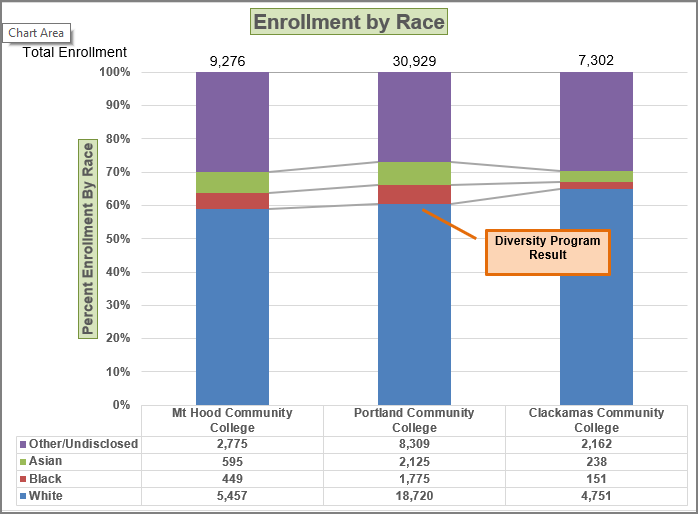
\includegraphics[width=\maxwidth{.95\linewidth}]{gfx/ch04_fig42}
	\caption{Completed Stacked Column Chart}
	\label{04:fig42}
\end{figure}


\begin{center}
	\begin{sklbox}{Skill Refresher}
		\textbf{Adding Series Lines}
		\\
		\begin{itemize}
			\setlength{\itemsep}{0pt}
			\setlength{\parskip}{0pt}
			\setlength{\parsep}{0pt}
			
			\item Click anywhere on the chart area.
			\item Click the \fmtRibbonTab{Layout} tab of the ribbon.
			\item Click the \fmtRibbonButton{Lines} button in the \fmtRibbonGroup{Analysis} group of commands.
			\item Click the \fmtPopupButton{Series Lines} option from the drop-down list.
			
		\end{itemize}
	\end{sklbox}
\end{center}

\begin{center}
	\begin{sklbox}{Skill Refresher}
		\textbf{Adding Annotations}
		\\
		\begin{itemize}
			\setlength{\itemsep}{0pt}
			\setlength{\parskip}{0pt}
			\setlength{\parsep}{0pt}
			
			\item Click anywhere on the chart area.
			\item Click the \fmtRibbonTab{Insert} tab of the ribbon.
			\item Click the \fmtRibbonButton{Text Box} button in the \fmtRibbonGroup{Text} group of commands.
			\item Click and drag the size of the text box needed on the chart.
			\item Apply any desired format changes from the Home tab of the ribbon.
			\item Type the desired text.
			
		\end{itemize}
	\end{sklbox}
\end{center}

\begin{center}
	\begin{infobox}{Integrity Check}
		\textbf{Annotations and Axis Titles}
		\\
		\\
		Although adding annotations and axis titles can be a tedious process, doing so maintains a high level of integrity for charts. People can misinterpret the message being conveyed by the chart if they make inaccurate assumptions about the values displayed. Axis titles and annotations help prevent readers from making false assumptions and ensure that readers see the most accurate representation of the message being conveyed by the chart.		
	\end{infobox}
\end{center}

\begin{center}
	\begin{tkwbox}{Key Take-Aways}
		\textbf{Save}
		\\
		\begin{itemize}
			\setlength{\itemsep}{0pt}
			\setlength{\parskip}{0pt}
			\setlength{\parsep}{0pt}

			\item Applying appropriate formatting techniques is critical for making a chart easier to read.
			\item Many formatting commands in the \fmtRibbonTab{Home} tab of the ribbon can be applied to a chart.
			\item To change the number format for a data label, use the \fmtPopupBox{Number} section in the \fmtPopupBox{Format Data Labels} dialog box. Note that Number format commands in the \fmtRibbonTab{Home} tab of the ribbon cannot be used for a data label.
			\item To change the number format for the values on the Y axis, and the X axis in the case of a scatter chart, use the \fmtPopupBox{Number} section of the \fmtPopupBox{Format Axis} dialog box. Note that Number format commands in the \fmtRibbonTab{Home} tab of the ribbon cannot be used for axis labels.
			\item Axis titles and annotations help prevent false assumptions from being made and ensure that the reader sees the most accurate representation of the information presented on a chart.
			
		\end{itemize}
	\end{tkwbox}
\end{center}

\section{Using Charts With Microsoft® Word® and Microsoft® Powerpoint®}

\begin{center}
	\begin{objbox}{Learning Objectives}
		\begin{itemize}
			\setlength{\itemsep}{0pt}
			\setlength{\parskip}{0pt}
			\setlength{\parsep}{0pt}

			\item Learn how to paste an image of an Excel chart into a Word document.
			\item Learn how to paste a link to an Excel chart into a PowerPoint slide.
			
		\end{itemize}
	\end{objbox}
\end{center}

Charts that are created in Excel are commonly used in Microsoft Word documents or for presentations that use Microsoft PowerPoint slides. Excel provides options for pasting an image of a chart into either a Word document or a PowerPoint slide. A link can also be set up between Excel and Word or PowerPoint charts so that if the data changes in the Excel file it is automatically reflected in the Word or PowerPoint files. Both methods of sharing a chart are covered in this section.

\subsection{Pasting a Chart Image Into Word}

This exercise needs two files:

\begin{itemize}
	\item The Excel spreadsheet used in this chapter: \fmtWorkbookName{CH4 Charting}.
	\item This Word document: \fmtWorkbookName{CH4 Diversity}
\end{itemize}

Excel charts can be valuable tools for explaining quantitative data in a written report. Reports that address business plans, public policies, budgets, and so on all involve quantitative data. For this example, assume that the \fmtWorksheetName{Change in Enrollment Statistics Spend Source} stacked column chart is being used in a student's written report (see Figure \ref{04:fig45}). The following steps demonstrate how to paste an image, or picture, of this chart into a Word document.

\begin{enumerate}
	\item Open \fmtWorkbookName{CH4 Diversity}. Save it as \fmtWorkbookName{CH4 Diversity in Enrollment in Community Colleges}.
	\item Click below the figure heading in the Word document that reads: \textit{Figure 1: Enrollment by Race}. The image of the stacked column chart will be placed below this heading.
	\item If needed, open the Excel file used in this chapter,  (\fmtWorkbookName{CH4 Charting}). Activate the \fmtPopupBox{Enrollment by Race} chart in the \fmtWorksheetName{Enrollment by Race Chart} sheet.
	\item Click the down arrow on the \fmtRibbonButton{Copy} button in the \fmtRibbonTab{Home} tab of the ribbon. Select \fmtRibbonButton{Copy as Picture},
	\item Select \fmtPopupButton{OK} --- Accepting the \textit{Copy Pictures} defaults:
	
	\begin{itemize}
		\item As shown on Screen
		\item Picture
	\end{itemize}	

	\item Go back to the \fmtWorkbookName{CH4 Diversity in Enrollment in Community Colleges} Word document by clicking the file in the taskbar.
	\item Confirm that the insertion point is below the \textit{Figure 1: Enrollment by Race} heading (see Figure \ref{04:fig43}) and click the \fmtRibbonButton{Paste} button in the \fmtRibbonTab{Home} tab of the ribbon (or press \fmtKeystroke{Crtl}+\fmtKeystroke{V}).
\end{enumerate}

\begin{figure}[H]
	\centering
	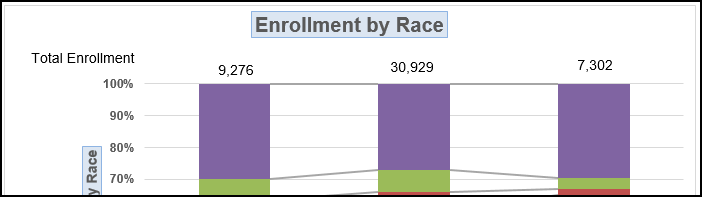
\includegraphics[width=\maxwidth{.95\linewidth}]{gfx/ch04_fig43}
	\caption{Paste Picture in Word}
	\label{04:fig43}
\end{figure}

Unfortunately, the picture is so big that it overlaps the next page. Use this procedure to change its size.

\begin{enumerate}
	\item Click anywhere on the picture to activate it.
	\item Click the \fmtRibbonTab{Format} tab under the \fmtRibbonGroup{Picture Tools} section of the ribbon (see Figure \ref{04:fig44}).
	\item Click the down arrow on the \fmtRibbonButton{Shape Width} button in the \fmtRibbonGroup{Size} group of commands. Continue to click the down arrow until the width of the picture is $ 5.4 $ inches. As the width is reduced the height is automatically reduced. (The height should be about $ 3.92 $ inches)
	\item To center the chart on the page, make sure the chart is activated. Then go to the \fmtRibbonTab{Home} tab, to the \fmtRibbonGroup{Paragraph} group, and select \fmtRibbonButton{Center}.
	\item Save the document.
\end{enumerate}

\begin{figure}[H]
	\centering
	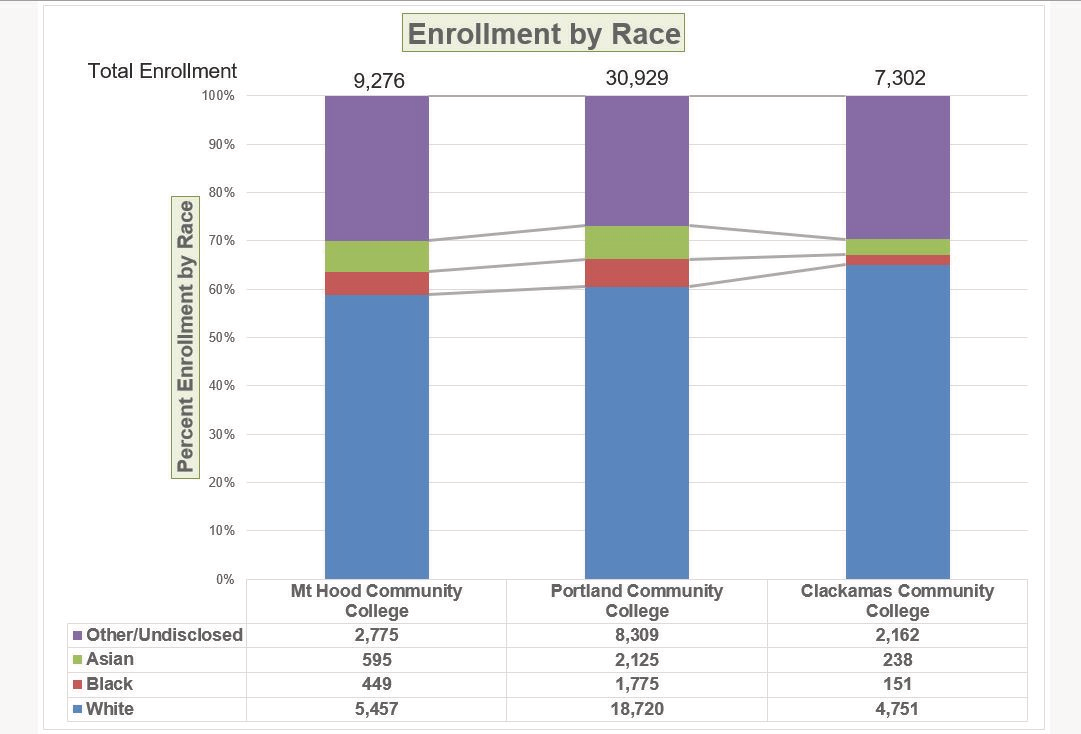
\includegraphics[width=\maxwidth{.95\linewidth}]{gfx/ch04_fig44}
	\caption{Changing the Size of a Picture in Word}
	\label{04:fig44}
\end{figure}

Figure \ref{04:fig45} shows the final appearance of the \fmtPopupBox{Enrollment by Race Source} chart pasted into a Word document. 

\begin{center}
	\begin{infobox}{Note}
		\textbf{Resizing Images}
		\\
		\\
		It is best to use either the \fmtRibbonButton{Shape Width} or \fmtRibbonButton{Shape Height} buttons to reduce the size of an embedded chart. Using either button automatically reduces both height and width in proper proportion. If the sizing handles are used, hold the \fmtKeystroke{Shift} key while clicking and dragging on a corner sizing handle to keep the chart in proper proportion.
	\end{infobox}
\end{center}

\begin{figure}[H]
	\centering
	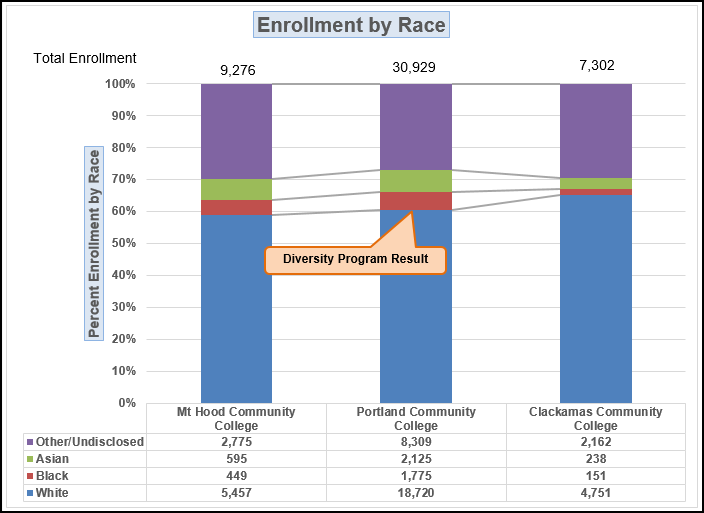
\includegraphics[width=\maxwidth{.95\linewidth}]{gfx/ch04_fig45}
	\caption{Final Appearance of Pasting a Chart Image into Word}
	\label{04:fig45}
\end{figure}

\begin{center}
	\begin{sklbox}{Skill Refresher}
		\textbf{Pasting a Chart Image into Word}
		\\
		\begin{itemize}
			\setlength{\itemsep}{0pt}
			\setlength{\parskip}{0pt}
			\setlength{\parsep}{0pt}

			\item Activate an Excel chart and click the \fmtRibbonButton{Copy} button in the \fmtRibbonTab{Home} tab of the ribbon.
			\item Click on the location in the Word document where the Excel chart will be pasted.
			\item Click the down arrow of the \fmtRibbonButton{Paste} button in the \fmtRibbonTab{Home} tab of the ribbon.
			\item Click the \fmtRibbonButton{Picture} option from the drop-down list.
			\item Click the \fmtRibbonTab{Format} tab in the \fmtRibbonGroup{Picture Tools} section of the ribbon.
			\item Resize the picture by clicking the up or down arrow on the \fmtRibbonButton{Shape Width} or \fmtRibbonButton{Shape Height} buttons.
			
		\end{itemize}
	\end{sklbox}
\end{center}

\subsection{Pasting a Linked Chart Image Into Powerpoint}

This exercise requires two files:

\begin{itemize}
	\item The Excel spreadsheet used in this chapter: \fmtWorkbookName{CH4 Charting}
	\item A PowerPoint file: \fmtWorkbookName{CH4 Diversity}
\end{itemize}

Microsoft PowerPoint is perhaps the most commonly used tool for delivering live presentations. The charts used in a live presentation are critical for efficiently delivering ideas to an audience. Similar to written documents, a wide range of presentations may require the explanation of quantitative data. This demonstration includes a PowerPoint slide that could be used in a presentation. The \fmtPopupBox{Enrollment by Race} chart will be pasted into this PowerPoint slide. However, instead of pasting an image, as demonstrated in the Word document above, a link will be established to the Excel file. As a result, if the chart in the Excel file is changed that change will be reflected in the PowerPoint file. The following steps explain how to link these two files.

\begin{enumerate}
	\item Open \fmtWorkbookName{CH4 Diversity.pptx} and save it as \fmtWorkbookName{CH4 Diversity in Enrollment in Community Colleges}.
	\item Navigate to Slide $ 6 $ – Diversity in Enrollment. This is the slide where the linked chart will be placed.
	\item If needed, open the Excel file used in this chapter, \fmtWorkbookName{CH4 Charting}. Activate the \fmtPopupBox{Enrollment by Race} chart in the \fmtWorksheetName{Enrollment by Race Chart} sheet.
	\item Click the down arrow on the \fmtRibbonButton{Copy} button in the \fmtRibbonTab{Home} tab of the ribbon. Select \fmtRibbonButton{Copy} (\textit{NOT} Copy as Picture.)
	\item Go back to the \fmtWorkbookName{CH4 Diversity in Enrollment in Community Colleges} presentation by clicking the file in the taskbar.
	\item Make sure Slide 6, Diversity in Enrollment, is still active. Click on the outside edge of the empty prompt box on the right.
	\item Click the down arrow below the \fmtRibbonButton{Paste} button in the \fmtRibbonTab{Home} tab of the ribbon in the PowerPoint file.
	\item Hover over each of the Paste Options until \fmtRibbonButton{Keep Source Formatting \& Link Data} is highlighted (see Figure \ref{04:fig46}). Select this option. This pastes an image of the Excel chart into the PowerPoint slide. In addition, a link is created so that any changes made to the chart (in Excel) appear on the PowerPoint slide.
\end{enumerate}

\begin{figure}[H]
	\centering
	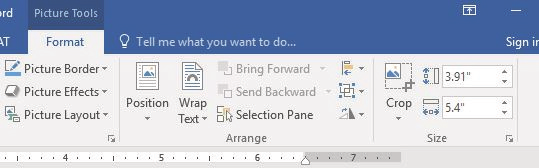
\includegraphics[width=\maxwidth{.95\linewidth}]{gfx/ch04_fig46}
	\caption{Creating a Link to an Excel Chart in PowerPoint}
	\label{04:fig46}
\end{figure}

Next, the chart needs to be cleaned up a bit. First, apply a different chart style.

\begin{enumerate}
	\item Click anywhere in the plot area of the column chart pasted into the PowerPoint slide. The same Chart Tools tabs found in Excel are added to the ribbon (see Figure \ref{04:fig47}). 
	\item On the \fmtRibbonTab{Design} tab, select Style $ 8 $ in the \fmtRibbonGroup{Chart Style} group.
\end{enumerate}

\begin{figure}[H]
	\centering
	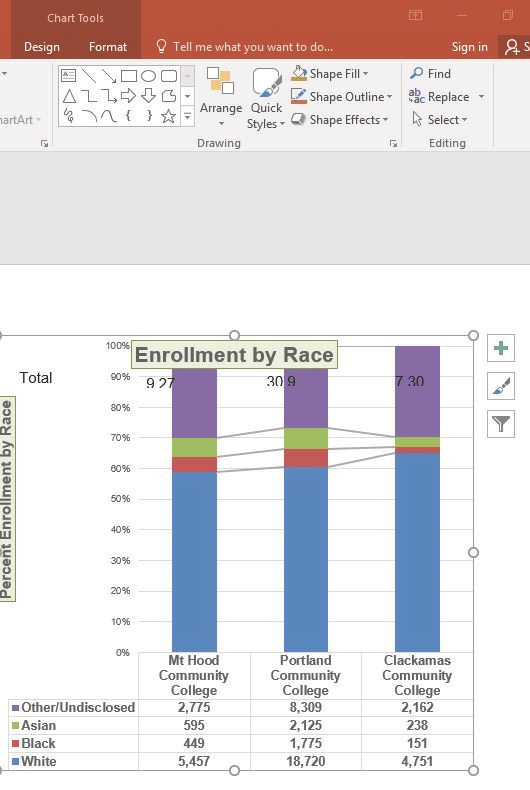
\includegraphics[width=\maxwidth{.95\linewidth}]{gfx/ch04_fig47}
	\caption{Modifying an Excel Chart Pasted into a PowerPoint Slide}
	\label{04:fig47}
\end{figure}

Linking this chart caused trouble with the text boxes, so delete them.

\begin{enumerate}
	\item Select each text box by clicking on the outside edge of the text box with the four-headed arrow.
	\item Press the \fmtKeystroke{Delete} key. Be sure that the insertion point is \textit{NOT} blinking inside the text box. If it is, the contents of the text box will be edited instead of deleting the complete text box.
\end{enumerate}

The benefit of adding this chart to the presentation as a link is that it will automatically update when the data in the linked spreadsheet file is changed.

\begin{enumerate}
	\item Return to \fmtWorkbookName{CH4 Charting Excel}.
	\item Select the \fmtWorksheetName{Enrollment Statistics} worksheet (the one with the Enrollment data.) Change the value in cell \fmtCellLocation{D3} to $ 1000 $ to change the number of white students at Clackamas Community College to $ 1000 $. This is not true but is a large enough change to see the result in the linked charts.
	\item Select the \fmtWorksheetName{Enrollment by Race Chart} worksheet. Notice how the chart has changed.
	\item Return to the \fmtWorkbookName{Diversity in Enrollment in Community Colleges} PowerPoint file by clicking the file in the taskbar.
	\item On Slide $ 6 $, notice that the chart was updated to reflect the change in enrollment (see Figure \ref{04:fig48}).
	\item If the chart has not changed, be sure that the chart is selected, click the \fmtRibbonTab{Design} tab in the \fmtRibbonGroup{Chart Tools} section of the ribbon, then click the \fmtRibbonButton{Refresh Data} button. The change made in the Excel workbook is now reflected on the PowerPoint slide.
	\item If that still does not work, check to see if a ``normal'' link was created instead instead of a ``Paste'' Link. If so, delete the chart and follow the steps again from the beginning of this section.
	\item Save all files. They will be submitted at the end of the next section.
\end{enumerate}

Figure \ref{04:fig48} shows the appearance of the column chart after the change was made in the \fmtWorksheetName{Enrollment Statistics} worksheet in the Excel file. Note that the \fmtPopupBox{Data Chart} at the bottom also reflects the new number. The change that was made in the Excel file will appear in the PowerPoint file after clicking the \fmtRibbonButton{Refresh }Data button.

\begin{figure}[H]
	\centering
	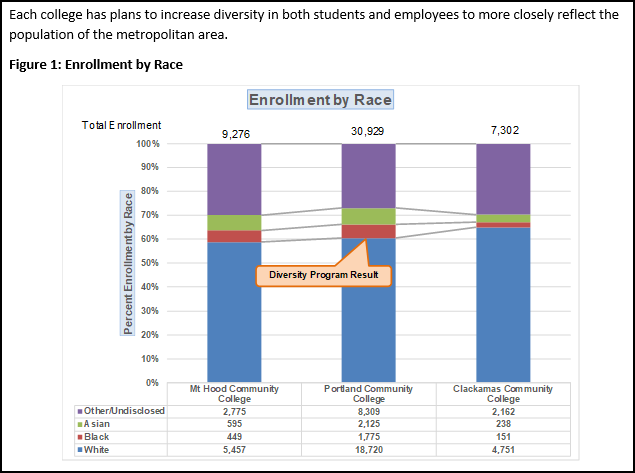
\includegraphics[width=\maxwidth{.95\linewidth}]{gfx/ch04_fig48}
	\caption{Styled and Updated Chart}
	\label{04:fig48}
\end{figure}

\begin{center}
	\begin{sklbox}{Skill Refresher}
		\textbf{Pasting a Linked Chart Image into PowerPoint}
		\\
		\begin{itemize}
			\setlength{\itemsep}{0pt}
			\setlength{\parskip}{0pt}
			\setlength{\parsep}{0pt}
			
			\item Activate an Excel chart and click the \fmtRibbonButton{Copy} button in the \fmtRibbonTab{Home} tab of the ribbon.
			\item Click in the PowerPoint slide where the Excel chart will be pasted.
			\item Click the down arrow of the \fmtRibbonButton{Paste} button in the \fmtRibbonTab{Home} tab of the ribbon.
			\item Click the \fmtRibbonButton{Keep Source Formatting \& Link Data} option from the drop-down list.
			\item Click the \fmtRibbonButton{Refresh Data} button in the \fmtRibbonTab{Design} tab of the ribbon to ensure any changes in the Excel file are reflected in the chart.
			
		\end{itemize}
	\end{sklbox}
\end{center}

\begin{center}
	\begin{infobox}{Integrity Check}
		\textbf{Refreshing Linked Charts in PowerPoint and Word}
		\\
		\\
		When creating a link to a chart in Word or PowerPoint, the data must be refreshed when there are changes in the Excel workbook. This is especially true if the changes are made in the Excel file prior to opening the Word or PowerPoint file that contains a link to a chart. To refresh the chart, make sure it is activated, then click the \fmtRibbonButton{Refresh Data} button in the \fmtRibbonTab{Design} tab of the ribbon. Forgetting this step can result in old or erroneous data being displayed in the chart.
	\end{infobox}
\end{center}

\begin{center}
	\begin{tkwbox}{Key Take-Aways}
		\textbf{Save}
		\\
		\begin{itemize}
			\setlength{\itemsep}{0pt}
			\setlength{\parskip}{0pt}
			\setlength{\parsep}{0pt}

			\item When pasting an image of an Excel chart into a Word document or PowerPoint file, use the \fmtPopupButton{Picture} option from the \fmtPopupBox{Paste} drop-down list of options to make it act as an image. Note that if the underlying data is updated the picture is not changed if it has been pasted as an image.
			\item When creating a link to a chart in Word or PowerPoint, the data may need to be refreshed if changes are made in the originating spreadsheet. 
					
		\end{itemize}
	\end{tkwbox}
\end{center}

\begin{center}
	\begin{infobox}{Integrity Check}
		\textbf{Severed Link?}
		\\
		\\
		When creating a link to an Excel chart in Word or PowerPoint, the Excel workbook must stay in its original location on the computer or network. If the workbook is moved or deleted, an error message will be generated when the link in the Word or PowerPoint file is updated. An error is also generated if the Excel workbook is saved on a network drive that the computer cannot access. These errors occur because the link to the Excel workbook has been severed. Therefore, if a USB drive is being used for a presentation then all of the linked Excel workbooks must be moved to the USB drive before establishing the Word or PowerPoint link.
	\end{infobox}
\end{center}

\section{Preparing to Print}

\begin{center}
	\begin{objbox}{Learning Objectives}
		\begin{itemize}
			\setlength{\itemsep}{0pt}
			\setlength{\parskip}{0pt}
			\setlength{\parsep}{0pt}

			\item Review each worksheet in a workbook in Print Preview.
			\item Modify worksheets as needed to professionally print data and charts.
			
		\end{itemize}
	\end{objbox}
\end{center}

This section considers each of the worksheets created in the previous sections. Since these worksheets contain a combination of data and charts, there are specific things to watch for when they are printed.

A good start point is to look at each worksheet in Print Preview in Backstage View. Then make any necessary changes, such as changing the orientation and scaling, or moving charts around on the worksheet. To make sure that no worksheets are missed, review them in the order they appear in the tabs.

\subsection{Previewing Chart Sheets for Printing}

Data file: \fmtWorkbookName{CH4 Charting}.

The first worksheet, \fmtWorksheetName{Closing Prices}, is a chart sheet. This means that it contains only a chart with no data; but it still needs to be reviewed in Print Preview.

\begin{enumerate}
	\item Click on the \fmtWorksheetName{Closing Prices} worksheet tab.
	\item Go to Print Preview by clicking \fmtRibbonButton{Print} in Backstage View.
	\item Notice that the chart will print on the entire page in Landscape orientation.
	\item There is nothing to change. Exit Backstage View.
\end{enumerate}

\subsection{Printing Worksheets With Data and Charts}

The next worksheet (\fmtWorksheetName{Stock Trend}) has both data and multiple charts. To print the data and the charts, the page setup will need some modification.

\begin{enumerate}
	\item Click on the \fmtWorksheetName{Stock Trend} worksheet tab.
	\item Go to Print Preview by clicking \fmtRibbonButton{Print} in Backstage View.
	\item Notice that this worksheet is currently printing on seven pages.
	\item Click through each page and note the following.

	\begin{itemize}
		\item The data is split between the first and third pages.
		\item The line chart starts on the first page, but part of it is also on the second page.
		\item The double-line chart starts on the third page and then finishes on the fifth page.
		\item The fourth and sixth pages are blank.
		\item The last page has a column of seemingly random numbers.
	\end{itemize}

	\item Exit Backstage View.
\end{enumerate}

The first thing to do is remove the numbers that are appearing on page $ 7 $. To do this, hide the column where they are stored. It is important to hide the column instead of deleting the numbers in case they are being utilized somewhere else in the workbook.

\begin{enumerate}
	\item Scroll to the right on the worksheet until the numbers in column AH are visible.
	\item Click anywhere in column AH.
	\item On the \fmtRibbonTab{Home} ribbon, click the \fmtRibbonButton{Format} button in the \fmtRibbonGroup{Cells} group.
	\item In the \fmtRibbonGroup{Visibility} section, select \fmtRibbonButton{Hide \& Unhide} then select \fmtRibbonButton{Hide Columns} (see Figure \ref{04:fig49}).
	\item The visible column headings should now go from AG to AI.
	\item Return to Print Preview in Backstage View to see the changes to the printed worksheet.
	\item Notice that there are now five pages. The data and charts are still splitting across multiple pages, but the numbers in column AH are no longer going to print.
	\item Remain in Backstage View for the next steps.
\end{enumerate}

\begin{figure}[H]
	\centering
	\includegraphics[width=\maxwidth{.95\linewidth}]{gfx/ch04_fig49}
	\caption{Hide Columns in Format Menu}
	\label{04:fig49}
\end{figure}

The data is still split between pages 2 and 3, and the charts are splitting oddly as well. The first step to fix these issues is to change the page orientation and scaling.

\begin{enumerate}
	\item While still in Backstage View, change the page orientation to \fmtRibbonButton{Landscape} (use the Orientation drop-down menu in the Settings section).
	\item This puts all of the data on one sheet, but the charts are still split between multiple pages.
	\item Change the page scaling to \fmtRibbonButton{Fit Sheet on One Page} (use the \fmtRibbonButton{Scaling} drop-down menu in the \fmtRibbonTab{Settings} section).
	\item This fits everything on one page, but it is too small to be able to read.
	\item Change the page scaling back to \fmtRibbonButton{No Scaling}.
\end{enumerate}

The next thing to try is moving one, or both, of the charts. In order to move the charts, exit out of Backstage View.

\begin{enumerate}
	\item Exit Backstage View.
	\item Switch to the \fmtRibbonTab{View} ribbon and then select \fmtRibbonButton{Page Break Preview}. The screen should look similar to Figure \ref{04:fig50}. (Remember that the dotted blue lines indicate automatic page breaks.)
	\item Move the \fmtPopupBox{24 Month Comparison} (double-line) chart closer to the top of its page.
	\item Move the \fmtPopupBox{May 2014-2015 Trend for NASDAQ Sales Volume} (line chart) so that it is under the \fmtPopupBox{24 Month Comparison} chart.
	\item The link to the data source is still at the bottom of page 2 (in \fmtCellLocation{A50:A51}) so it needs to move from \fmtCellLocation{A50:A51} to \fmtCellLocation{M31:M32}.
	\item The screen should look similar to Figure \ref{04:fig51}.
\end{enumerate}

\begin{figure}[H]
	\centering
	\includegraphics[width=\maxwidth{.95\linewidth}]{gfx/ch04_fig50}
	\caption{Page Break Preview before moving the charts in Step 3}
	\label{04:fig50}
\end{figure}

\begin{figure}[H]
	\centering
	\includegraphics[width=\maxwidth{.95\linewidth}]{gfx/ch04_fig51}
	\caption{Page Break Preview after moving the charts and text}
	\label{04:fig51}
\end{figure}

The data source link text should not print on its own page, but there is no room to move it onto the same page as the charts. To fix this, remove the automatic page break between the charts and the text in \fmtCellLocation{M31:M32}.

\begin{enumerate}
	\item Place the pointer on the horizontal blue dashed line (automatic page break) between the line chart and the Data Source link text.
	\item When the pointer changes to the double arrow (pointing up and down), drag the page break down into the gray area. This removes the page break.
	\item If the vertical automatic page break between columns L and M moves, drag it back between columns L and M. This will make it a solid blue line, which will no longer adjust automatically.
	\item The screen should now look like Figure \ref{04:fig52}.
\end{enumerate}

\begin{figure}[H]
	\centering
	\includegraphics[width=\maxwidth{.95\linewidth}]{gfx/ch04_fig52}
	\caption{Page Break Preview after removing a page break}
	\label{04:fig52}
\end{figure}

Now complete one final check of this worksheet in Print Preview.

\begin{enumerate}
	\item Go to Print Preview and look at both pages. Page $ 1 $ should contain just the data and page $ 2 $ should have both charts and the Data Source link text.
	\item Exit Backstage View and save the workbook.
\end{enumerate}

\subsection{Preview Remaining Worksheets for Printing}

There are four remaining worksheets to be reviewed. Some of them will need minor changes and some will not need any changes. Preview each one and make the changes specified.

\begin{enumerate}
	\item \fmtWorksheetName{All Excel Classes}: this is a chart sheet, so it should not need any changes.
	\fmtWorksheetName{Grade Distribution}: the chart is split across two pages. Fix this by changing the orientation (Landscape) and scaling (Fit Sheet on One Page).
	\fmtWorksheetName{Enrollment by Race Chart}: this is a chart sheet, so it should not need any changes.
\end{enumerate}

\subsection{Printing a Chart Only}

Sometimes a worksheet may have both data and a chart but only the chart should print. That is the case with the \fmtWorksheetName{Enrollment Statistics} worksheet.

\begin{enumerate}
	\item Switch to the \fmtWorksheetName{Enrollment Statistics} worksheet.
	\item Select the chart.
	\item Go to Print Preview. Only the chart is printing. (If it shows the data printing along with the chart, exit Backstage View and be sure to select just the chart on the worksheet.)
	\item If needed, change the orientation to Landscape. This orientation looks better when printing just a chart.
	\item Exit Backstage View.
\end{enumerate}

\subsection{Hiding a Worksheet}

It is possible to hide an entire worksheet so it will not print nor will anyone looking at the workbook see it. Keep in mind that this is not a security feature since someone can simply unhide the sheet, but it makes it easier to focus on the data and charts that are important. For this section, hide the \fmtWorksheetName{Enrollment by Race Chart} sheet.

1. Right-click on the \fmtWorksheetName{Enrollment by Race Chart} tab.
2. Select Hide from the menu that appears. The \fmtWorksheetName{Enrollment by Race Chart} sheet should no longer be visible.
3. To unhide the worksheet, right-click on any other worksheet tab and select Unhide from the menu. A list of hidden worksheets will be displayed. Select the \fmtWorksheetName{Enrollment by Race Chart} and click \fmtPopupButton{OK}.
4. Save the \fmtWorkbookName{CH4 Charting} workbook.
5. Compare all of the worksheets with the self-check answer key.
6. Submit all three files from this chapter (\fmtWorkbookName{CH4 Charting.xlsx}, \fmtWorkbookName{CH4 Diversity in Enrollment in Community Colleges.docx}, and \fmtWorkbookName{CH4 Diversity in Enrollment in Community Colleges.pptx}).

\section{Chapter Practice}

Although Excel is primarily used in business and scientific applications, it is useful in other areas of study as well. In these exercises, Excel is used to create charts using historical, health, and social justice data.

\subsection{Charting Historical Data (Comprehensive Review)}

\textit{Data File: PR4 Data}

Excel is an excellent tool for helping to display historical date. This exercise examines information on minimum wage data and life expectancy.

\subsubsection{Task1 – National Minimum Wage in the Us – 1960-2014}

Since the beginning of the previous century, the United States has set a minimum wage, in order to set a ``floor'' beneath which wages cannot fall. Most states have set their own minimum wages, but none are lower than the national minimum wage. To learn more about the national minimum wage, look at \url{https://en.wikipedia.org/wiki/Minimum_wage_in_the_United_States}

\begin{enumerate}
	\item Open the file named \fmtWorkbookName{PR4 Data} and then Save As \fmtWorkbookName{PR4 Historical Data}.
	\item On the \fmtWorksheetName{Minimum Wage} worksheet, select the range \fmtCellLocation{B4:C60}.
	\item Select the \fmtRibbonTab{Insert} tab, then the \fmtRibbonButton{Recommended Chart} tool in the \fmtRibbonGroup{Charts} group. \fmtRibbonButton{Recommended Charts} allows users to first see how selected data would be represented on a variety of chart types before committing to a particular type of chart. Being able to see the data as it would look in a variety of charts helps when selecting the kind of chart that best matches the data. It does a particularly good job when using dates or years as labels, though sometimes Excel gets confused and thinks that dates are part of the data instead of labels.
	\item Select the first Line chart. Press \fmtPopupButton{OK}.
	\item The line chart is embedded in the \fmtWorksheetName{Minimum Wage} worksheet.
	\item Make sure that the upper left corner of the chart is in the upper left corner of \fmtCellLocation{E4}. The lower right corner is in the lower right corner of \fmtCellLocation{M20}.
	\item Adjusting the chart title: Click the chart title once. Then click in front of the first letter. A blinking cursor appears in front of the letter. This allows the title of the chart to be modified.
	\item Type the following in front of the first letter in the chart title: \fmtTyping{US National}.
	\item While the chart is still selected, select the \fmtRibbonTab{Design} tab and find the \fmtRibbonGroup{Chart Styles} group in the middle of the ribbon. If necessary, press the More button to see the available styles.
	\item Float the cursor over the available styles to see how each will affect the chart. Select Style $ 4 $.
	\item The years across the X (category) axis are a little hard to read. Select the labels so there is a box surrounding the list of years. On the \fmtRibbonTab{Home} tab, in the \fmtRibbonGroup{Alignment} Group, select the \fmtRibbonButton{Orientation} tool. Select \fmtPopupButton{Angle Counter Clockwise}.
	\item Prepare the \fmtWorksheetName{Minimum Wage} worksheet for printing by changing the scaling to Fit Sheet on One Page.
\end{enumerate}

\subsubsection{Task2 – Oregon: Projected Life Expectancy at Birth}

In the past $ 40 $ years, between $ 1970 $ and $ 2010 $, life expectancy for Oregon men improved by $ 8.7 $ years and for women by $ 5.5 $ years. Oregon's life expectancy has remained slightly higher than the U.S. average. The life expectancy will continue to improve for both men and women. However, the gain for men has been outpacing the gain for women. Consequently, the difference between men's and women's life expectancies has continued to shrink. This data was found at \url{https://www.oregon.gov/das/OEA/Documents/OR_pop_trend2012.pdf}

\begin{enumerate}
	\item On the \fmtWorkbookName{Life Expectancy} sheet, select \fmtCellLocation{A5:B11}
	\item Press \fmtKeystroke{F11}
	\item This creates a column chart and puts it on a separate sheet.
	\item Double click the chart sheet tab, change the name to \fmtTyping{Men}.
	\item Take a good look at this chart. It is not what was expected. Excel has made a mistake and charted the Birth Year information as though it was data, instead of using it to label the bottom (category) axis. That needs to be fixed.
	\item With the chart selected, go to the \fmtRibbonTab{Design} tab, and select the \fmtRibbonButton{Select Data} tool. This opens the \fmtPopupBox{Select Data Source} dialog box. The box at the top tells us the range that was selected, which looks fine. 
\end{enumerate}
	
The Legend Entries need to be corrected to fix the issue with the data series (columns). Also, the Horizontal Axis Labels are just a series of default numbers. They need to be the range that contains the years.

\begin{enumerate}[resume]
	\item In the \fmtPopupBox{Legend Entries}, click in the small box in front of \fmtPopupButton{Birth Year} to remove the check mark. This will remove the Birth Year as a data series on the chart.
	\item In the \fmtPopupBox{Horizontal (Category) Axis Labels} box, press the \fmtPopupButton{Edit} button. This will open the \fmtPopupBox{Axis Labels} dialog box. Press the \fmtPopupButton{Select range} button.
	\item Navigate to the \fmtRibbonTab{Life Expectancy} tab and select \fmtCellLocation{A6:A11}. After \fmtTyping{=’Life Expectancy’!$A$6:$A$11} is displayed in the box, press the Select Range button. Press \fmtPopupButton{OK}. Press \fmtPopupButton{OK} a second time.
	\item Change the chart title so that it reads: \fmtTyping{Life Expectancy for Oregon Men}.
	\item Remove the Legend from the bottom of the chart by right-clicking on it and selecting \fmtPopupButton{Delete} from the context menu.
	\item Return to the \fmtRibbonTab{Life Expectancy} tab, select \fmtCellLocation{A5:A11}, \fmtCellLocation{C5:C11} (Select the first range, hold down the \fmtKeystroke{Ctrl} key, select both noncontiguous ranges at the same time.
	\item Repeat steps $ 2 $-$ 11 $ above to create a matching chart for \textit{Life Expectancy for Oregon Women}.
	\item Return to the \fmtRibbonTab{Life Expectancy} tab, select \fmtCellLocation{A5:D11}.
	\item Use the \fmtRibbonButton{Recommended Charts} tool to create a simple line chart.
	\item Change the Chart Title to Oregon: \fmtTyping{Projected Life Expectancy at Birth}.
	\item The green line across the bottom of the chart represents the difference between men's and women's life expectancy. It is not very helpful as it is. Right click on the green line to open the pop up menu. Select \fmtPopupButton{Format Data Series}. In the \fmtPopupBox{Format Data Series} pane, under the \fmtPopupBox{Series Options} tab, select the radio button in front of \fmtPopupButton{Secondary Axis}.
	\item Close the \fmtPopupBox{Format Data Series} pane.
	\item Add a text box that explains the Difference calculation. While the chart is still selected:
	
	\begin{itemize}
		\item On the \fmtRibbonTab{Insert} tab, on the right side of the ribbon, find \fmtRibbonButton{Text}. Select the \fmtRibbonButton{Text Box} tool.
		\item Notice that the cursor has turned into a cross hair (thin black plus sign)
		\item Click once in the lower left corner of the chart. This creates a text box.
		\item Type the following into the text box: \fmtTyping{Difference = Female life expectancy minus male}.
		\item Move or resize the text box as desired.
	\end{itemize}
	
	\item Move or resize the chart so that it no longer is on top of the spreadsheet data.
	\item Use the \fmtRibbonButton{Chart Styles} tools to change the chart to something a bit more dramatic.
	\item Preview the Life Expectancy worksheet in Print Preview and make any necessary changes.
	\item Save the \fmtWorkbookName{PR4 Historical Data} workbook.
	\item Compare the final worksheet with the self-check answer key and then submit the \fmtWorkbookName{PR4 Historical Data} workbook as directed by the instructor.
\end{enumerate}

\section{Scored Assessment}

\subsection{Charting Social Justice Data (Comprehensive Review)}

\textit{Data File: SC4 Data}

\subsubsection{Task 1 International Incarceration Rates}

\begin{enumerate}
	\item Open the file named \fmtWorkbookName{SC4 Data} and then Save As \fmtWorkbookName{SC4 Social Justice}.
	\item On the \fmtWorksheetName{International} tab, use a function in cell \fmtCellLocation{D20} to find the average of the Individuals' incarcerated data.
	\item Create a bar chart that looks like Figure \ref{04:fig53}:
\end{enumerate}

\begin{figure}[H]
	\centering
	\includegraphics[width=\maxwidth{.95\linewidth}]{gfx/ch04_fig53}
	\caption{International Incarceration Rates}
	\label{04:fig53}
\end{figure}

\begin{enumerate}
	\item Move and or resize the chart so that it does not cover any of the data.
	\item In cell \fmtCellLocation{A25} write a brief note explaining why a bar (or column) chart is a better choice for this data than a pie chart.
	\item Set the Print Area so that everything prints, except for the explanation that was added in cell \fmtCellLocation{A25}.
	\item Preview the \fmtWorksheetName{International} worksheet in Print Preview and make any changes needed to print professionally on one page.
\end{enumerate}

\subsubsection{Task 2 Disenfranchisement Rate}

Felony disenfranchisement is the exclusion from voting of people otherwise eligible to vote (known as disfranchisement) due to conviction of a criminal offense, usually restricted to the more serious class of crimes: felonies. Jurisdictions vary as to whether they make such disfranchisement permanent or restore suffrage after a person has served a sentence or completed parole or probation. Affected individuals suffer ``collateral consequences'' including loss of access to jobs, housing, and other facilities.

Opponents have argued that such disfranchisement restricts and conflicts with principles of universal suffrage. It can affect civic and communal participation in general. For more information, see \url{https://en.wikipedia.org/wiki/Felony_disenfranchisement}.

On the \fmtWorksheetName{Disenfranchisement Rate} sheet, use the \fmtRibbonButton{Recommended Chart} tool to create the following three charts. Put each chart on its own individual sheet rather than an object in a spreadsheet.

\fmtWorksheetName{Chart1 — Felony Disenfranchisement Rate Washington}

\begin{figure}[H]
	\centering
	\includegraphics[width=\maxwidth{.95\linewidth}]{gfx/ch04_fig54}
	\caption{Felony Disenfranchisement Rate Washington}
	\label{04:fig54}
\end{figure}

\fmtWorksheetName{Chart2 — Felony Disenfranchisement Rate Oregon}

\begin{figure}[H]
	\centering
	\includegraphics[width=\maxwidth{.95\linewidth}]{gfx/ch04_fig55}
	\caption{Felony Disenfranchisement Rate Oregon}
	\label{04:fig55}
\end{figure}

\fmtWorksheetName{Chart3 – Comparison – Oregon and Washington}

\begin{figure}[H]
	\centering
	\includegraphics[width=\maxwidth{.95\linewidth}]{gfx/ch04_fig56}
	\caption{Comparison of Oregon and Washington}
	\label{04:fig56}
\end{figure}

\begin{center}
	\begin{infobox}{Notes}
		\textbf{Chart 1}
		\\
		This is called a Clustered column chart in the Recommended charts tool, but it is really a combo chart where some data is displayed as columns and some as a line.
		
		Be sure to edit the Chart Title.
		
		Adjust the chart size to make it look like the illustration.
		
		Put the chart on its own individual sheet, do not leave it as an object on the spreadsheet.
	\end{infobox}
\end{center}

Take a look at both the Washington and Oregon charts. They are the same kind of chart, but they may look different because the data is a bit different. To make the charts more similar make sure that the vertical axes are the same in both charts. Format the left vertical (value) axis on both charts so that the Maximum is $ 20000 $ and the right vertical axis so that the Maximum is $ .20 $. Be sure that \textit{years} are used as labels on the horizontal axis instead of numbers like $ 1 $, $ 2 $, $ 3 $. Each of the three charts should be on separate sheets.

\begin{enumerate}
	\item Save all three charts when they are completed. 
	\item Preview the worksheet(s) in Print Preview and make any necessary changes for professional printing.
	\item Submit the \fmtWorkbookName{SC4 Social Justice} workbook as directed by the instructor.
\end{enumerate}